%%%%%%%%%%%%%%%%%%%%%%
%ndss and S&P
%\documentclass[conference]{IEEEtran}
%\pagestyle{plain}

%CCS
\documentclass[sigconf, anonymous]{acmart}
\fancyhf{} % Remove fancy page headers 
\fancyhead[C]{Anonymous submission \#9999 to ACM CCS 2021} % TODO: replace 9999 with your paper number
\fancyfoot[C]{\thepage}

\setcopyright{none} % No copyright notice required for submissions
\acmConference[Anonymous Submission to ACM CCS 2021]{ACM Conference on Computer and Communications Security}{Due 15 May 2019}{London, TBD}
\acmYear{2021}
\settopmatter{printacmref=false, printccs=true, printfolios=true} % We want page numbers on submissions


%%%%%%%%%%%%%%%%%%%%%%
% \usepackage{enumitem}
\usepackage{graphicx}
\usepackage{xcolor}
\usepackage{pifont}
% \usepackage[draft]{hyperref}
\usepackage{adjustbox}
\usepackage{caption}
\usepackage{subcaption}
\usepackage{mathtools}
\usepackage{mathrsfs}
\usepackage{xspace}
\usepackage{url}
\usepackage[mode=buildnew]{standalone}
\usepackage{tikz}
\usepackage{pifont}
\usepackage{wasysym}
\usepackage{booktabs}
\usepackage{multirow}
\usetikzlibrary{positioning, trees, arrows, calc, automata}
% \usepackage{enumitem}
\usepackage{cleveref}
\usepackage{mfirstuc}
\usepackage{pifont}
%\usepackage[font={small}]{caption}
%\usepackage{enumitem}
%\usepackage[shortlabels]{enumitem}
%\usepackage{cite}
%\usepackage{flushend}
%\usepackage{hyperref}
%\usepackage{caption}

% \usepackage[
% all=normal%
% ,floats=tight%
% ,paragraphs=tight%
% % ,wordspacing=tight
% %,mathspacing=tight
% %,mathdisplays=tight
% ]{savetrees}

%\hypersetup{draft}

%% tikz figure icon definitions
% \pgfdeclareimage[width=2cm]{enclave}{icons/enclave}
% \pgfdeclareimage[width=2cm]{enclave-yellow}{icons/sgx_red}
% \pgfdeclareimage[width=2cm]{enclave-red}{icons/sgx_yellow}
% \pgfdeclareimage[width=2cm]{server}{icons/server_contoured}
% \pgfdeclareimage[width=2cm]{blockchain}{icons/blockchain}
% \pgfdeclareimage[width=2cm]{user}{icons/persons/user/user}
% \pgfdeclareimage[width=2cm]{attacker}{icons/persons/burglar}
% \pgfdeclareimage[width=1cm]{phone}{icons/smartphone}
% \pgfdeclareimage[width=2cm]{computer}{icons/devices/client}

% \pgfdeclareimage[width=2cm]{memory}{icons/computerpack/013-ram}
% \pgfdeclareimage[width=1.4cm]{gpu}{icons/computerpack/002-vga}
% \pgfdeclareimage[width=1.4cm]{mouse}{icons/computerpack/017-mouse}
% \pgfdeclareimage[width=1.4cm]{keyboard}{icons/computerpack/024-keyboard}
% \pgfdeclareimage[width=1.4cm]{screen}{icons/computerpack/018-monitor-2}
% \pgfdeclareimage[width=1.4cm]{lan}{icons/computerpack/023-lan}
% \pgfdeclareimage[width=1.4cm]{lanred}{icons/computerpack/023-lan-red}

% \definecolor{col1}{RGB}{170, 72, 59}
% \definecolor{col2}{RGB}{170,114, 59}
% \definecolor{col3}{RGB}{ 38, 93,105}
% \definecolor{col4}{RGB}{ 44,127, 66}

\definecolor{col1}{HTML}{4398D1}
\definecolor{col2}{HTML}{FF4842}
\definecolor{col3}{RGB}{ 38, 93,105}
\definecolor{col4}{RGB}{ 44,127, 66}

\definecolor{greenc}{HTML}{64c37d}
\definecolor{redc}{HTML}{e13957}

\ifstandalone
    \newcommand{\icon}[1]{../icons/#1}
\else
    \newcommand{\icon}[1]{images/icons/#1}
\fi

\newcommand{\imgmemory}{
\includegraphics[width=2.0cm]{\icon{computerpack/013-ram}}}
\newcommand{\imggpu}{
\includegraphics[width=1.4cm]{\icon{computerpack/002-vga}}}
\newcommand{\imggpusmall}{
\includegraphics[width=1.0cm]{\icon{computerpack/002-vga}}}
\newcommand{\imgmouse}{
\includegraphics[width=1.4cm]{\icon{computerpack/017-mouse}}}
\newcommand{\imgkeyboard}{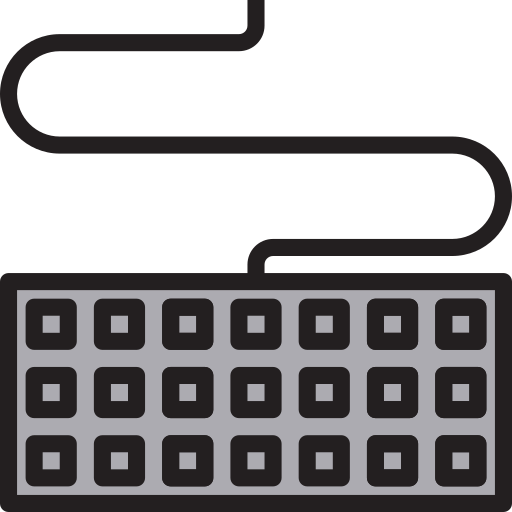
\includegraphics[width=1.4cm]{\icon{computerpack/024-keyboard}}}
\newcommand{\imgscreen}{\includegraphics[width=1.4cm]{\icon{computerpack/018-monitor}}}
\newcommand{\imglan}{
\includegraphics[width=1.4cm]{\icon{computerpack/023-lan}}}
\newcommand{\imglanred}{
\includegraphics[width=1.4cm]{\icon{computerpack/023-lan-red}}}
\newcommand{\imgcpu}{
\includegraphics[width=1.4cm]{\icon{computerpack/034-cpu}}}
\newcommand{\imgcpusmall}{
\includegraphics[width=1.0cm]{\icon{computerpack/034-cpu}}}

\newcommand{\imgdisplay}{\includegraphics[height=1.4cm]{\icon{computerpack/021-mobile}}}
\newcommand{\imgdisplaysmall}{\includegraphics[height=1.0cm]{\icon{computerpack/021-mobile}}}
\newcommand{\imgsim}{
\includegraphics[height=1.4cm]{\icon{computerpack/008-sim-card}}}
\newcommand{\imgsimsmall}{
\includegraphics[height=1.0cm]{\icon{computerpack/008-sim-card}}}
\newcommand{\imgsd}{
\includegraphics[height=1.4cm]{\icon{computerpack/011-sd-card}}}
\newcommand{\imgsdsmall}{
\includegraphics[height=1.0cm]{\icon{computerpack/011-sd-card}}}
\newcommand{\imgcamera}{\includegraphics[width=1.4cm]{\icon{computerpack/035-camera}}}
\newcommand{\imgcamerasmall}{\includegraphics[width=1.0cm]{\icon{computerpack/035-camera}}}

\newcommand{\imgenclave}{\includegraphics[width=2.0cm]{\icon{enclave}}}
\newcommand{\imgenclavesmall}{\includegraphics[width=1.4cm]{\icon{enclave}}}
\newcommand{\imgenclavesmaller}{\includegraphics[width=1.0cm]{\icon{enclave}}}
\newcommand{\imgenenclavered}{\includegraphics[width=2.0cm]{\icon{sgx_red}}}
\newcommand{\imgenenclaveredsmall}{\includegraphics[width=1.0cm]{\icon{sgx_red}}}
\newcommand{\imguser}{
\includegraphics[height=2.0cm]{\icon{persons/user/user}}}
\newcommand{\imgusersmall}{
\includegraphics[height=1.4cm]{\icon{persons/user/user}}}
\newcommand{\imgattacker}{
\includegraphics[width=2.0cm]{\icon{persons/burglar}}}
\newcommand{\imgattackersmall}{
\includegraphics[height=1.4cm]{\icon{persons/burglar}}}
\newcommand{\imgcomputer}{
\includegraphics[width=2.0cm]{\icon{devices/client}}}

\newcommand{\imglock}{\includegraphics[width=0.3cm]{\icon{lock-icon}}}
\newcommand{\imglocklarge}{\includegraphics[width=0.5cm]{\icon{lock-icon}}}
\newcommand{\imgkeyyellow}{\includegraphics[width=0.5cm]{\icon{key-yellow}}}
\newcommand{\imgkeyred}{\includegraphics[width=0.5cm]{\icon{key-red}}}
\newcommand{\imgkeyblue}{\includegraphics[width=0.5cm]{\icon{key-blue}}}
\newcommand{\imgcertred}{\includegraphics[width=0.5cm]{\icon{certificate-red}}}
\newcommand{\imgcertyellow}{\includegraphics[width=0.5cm]{\icon{certificate-yellow}}}
\newcommand{\imgcertblue}{\includegraphics[width=0.5cm]{\icon{certificate-blue}}}

\newcommand{\imgdevil}{\includegraphics[width=0.6cm]{\icon{devil}}}

\let\oldding\ding% Store old \ding in \oldding
\renewcommand{\ding}[2][1]{\scalebox{#1}{\oldding{#2}}}% Scale \oldding via optional argument

\newcommand{\zero}{\ding[1.2]{171}\xspace}
\newcommand{\one}{\ding[1.2]{172}\xspace}
\newcommand{\two}{\ding[1.2]{173}\xspace}
\newcommand{\three}{\ding[1.2]{174}\xspace}
\newcommand{\four}{\ding[1.2]{175}\xspace}
\newcommand{\five}{\ding[1.2]{176}\xspace}
\newcommand{\six}{\ding[1.2]{177}\xspace}
\newcommand{\seven}{\ding[1.2]{178}\xspace}
\newcommand{\eight}{\ding[1.2]{179}\xspace}
\newcommand{\nine}{\ding[1.2]{180}\xspace}
\newcommand{\ten}{\ding[1.2]{181}\xspace}

\newcommand{\risc}{RISC-V\xspace}
\newcommand{\ce}{controller enclave\xspace}
\newcommand{\ces}{controller enclave\xspace}
\newcommand{\Ce}{Controller enclave\xspace}
\newcommand{\Ces}{Controller enclave\xspace}
\newcommand{\app}{application enclave\xspace}
\newcommand{\App}{Application enclave\xspace}
\newcommand{\apps}{application enclaves\xspace}
\newcommand{\Apps}{Application enclaves\xspace}


\newcommand*\circled[1]{\tikz[baseline= (char.base)]{
            \node[shape=circle,draw,inner sep=0.3pt] (char) {\(#1\)};}}

\newcommand{\blue}[1]{\textcolor{black}{#1}}
\newcommand{\red}[1]{\textcolor{red}{#1}}


\newcommand{\figsaver}[0]{\vspace{-5pt}}
\newcommand{\parasaver}[0]{\vspace{-2pt}}

\newif\ifremoveall{}
\removealltrue{}

\ifremoveall{}
\newcommand{\aritra}[1]{\textbf{\emph{ #1 \colorbox{green}{[Aritra]}}}}
\newcommand{\ip}[1]{\textbf{\emph{ #1 \colorbox{cyan}{[Ivan]}}}}
\newcommand{\moritz}[1]{\textbf{\emph{ #1 \colorbox{yellow}{[Moritz]}}}}
\newcommand{\srdjan}[1]{\textbf{\emph{ #1 \colorbox{blue}{[Srdjan]}}}}
\newcommand{\todo}[1]{\textcolor{red}{TODO: \@#1}}
\newcommand{\todoref}{\textcolor{red}{[ref]}}
\newcommand{\citneed}{[\textcolor{red}{cit}] }
\else
\newcommand{\aritra}[1]{}
\newcommand{\ip}[1]{}
\newcommand{\moritz}[1]{}
\newcommand{\todo}[1]{}
\newcommand{\todoref}[1]{}
\newcommand{\citneed}[1]{}
\fi


\newcommand{\name}{\textsc{PIE}\xspace}
\newcommand{\tool}{\textsc{\name{} API}\xspace}
\newcommand{\device}{\textsc{Device}\xspace}

\newcommand{\usb}{\texttt{USB}\xspace}
\newcommand{\tls}{\texttt{TLS}\xspace}

\def\nameenclave{platform-wide enclave\xspace}
\def\Nameenclave{Platform-wide enclave\xspace}

\newcommand{\sphw}[0]{specialized hardware\xspace}
\newcommand{\Sphw}[0]{Specialized hardware\xspace}


%%%%%%%%%%%%%%%%%%%%%%
%savetrees
\usepackage[
all=normal,floats=tight
,paragraphs=tight
% ,wordspacing=tight
,mathspacing=tight
% ,mathdisplays=tight
]{savetrees}
%%%%%%%%%%%%%%%%%%%%%%

% \newcommand{\myparagraph}[1]{\par\emph{#1.}\xspace}
\newcommand{\myparagraph}[1]{\paragraph{#1}}

\newcounter{para}
% \newcommand{\mypara}[1]{\refstepcounter{para}\emph{\thepara}.\space\emph{#1}.\xspace}
\newcommand{\mypara}[1]{\refstepcounter{para}\paragraph{\thepara.\space{}#1}}
% \newcommand{\mypara}[1]{\paragraph{#1}}
%\newcommand\mypara{\par\refstepcounter{para}\thepara\space}

%------------------------------------------------------------------------------
%                                Space savers.
%------------------------------------------------------------------------------
% This mylist environment indents items, and saves less space than the above.
\newcounter{myctr}
\newenvironment{mylist}{\begin{list}{\arabic{myctr}.}
{\usecounter{myctr}
\setlength{\topsep}{1mm}\setlength{\itemsep}{0.5mm}
\setlength{\parsep}{0.5mm}
\setlength{\itemindent}{1mm}\setlength{\partopsep}{0mm}
\setlength{\labelwidth}{-2mm}
\setlength{\leftmargin}{0mm}}}{\end{list}}

\newenvironment{mylist_indent}{\begin{list}{\arabic{myctr}.}
{\usecounter{myctr}
\setlength{\topsep}{1mm}\setlength{\itemsep}{0.5mm}
\setlength{\parsep}{0.5mm}
\setlength{\itemindent}{1.5mm}\setlength{\partopsep}{1mm}
\setlength{\labelwidth}{-2mm}
\setlength{\leftmargin}{1mm}}}{\end{list}}

% Space saving List environment for itemizing.
\newenvironment{mybullet}{\begin{list}{\bullet}
{\setlength{\topsep}{1mm}\setlength{\itemsep}{0.5mm}
\setlength{\parsep}{0.5mm}
\setlength{\itemindent}{0mm}\setlength{\partopsep}{0mm}
\setlength{\labelwidth}{-2mm}
\setlength{\leftmargin}{0mm}}}{\end{list}}


% Break characters in the reference
\expandafter\def\expandafter\UrlBreaks\expandafter{\UrlBreaks
  \do\a\do\b\do\c\do\d\do\e\do\f\do\g\do\h\do\i\do\j
  \do\k\do\l\do\m\do\n\do\o\do\p\do\q\do\r\do\s\do\t
  \do\u\do\v\do\w\do\x\do\y\do\z\do\A\do\B\do\C\do\D
  \do\E\do\F\do\G\do\H\do\I\do\J\do\K\do\L\do\M\do\N
  \do\O\do\P\do\Q\do\R\do\S\do\T\do\U\do\V\do\W\do\X
  \do\Y\do\Z}
  
  


\newif\ifpaper
\papertrue

\newif\ifbold
\boldtrue

\newif\ifdesperatetime
%\desperatetimetrue

\graphicspath{{images/}}

\begin{document}
%\title{\name: Integrity Protection of User Input \\ for Remote Configuration of Safety-Critical Devices}
\title{\name: Integrity Protection of Keyboard Input for Security-Critical Web Services \\ (Long Paper)}


\maketitle
\keywords{Input integrity \and Web application security \and Embedded systems}
\begin{abstract}
Many security-critical web services are used from hosts that are standard PCs. For example, industrial control systems, medical devices, and home automation systems are often configured through web interfaces. Similarly, online banking payments and cryptocurrency transactions are often executed through web interfaces. In such cases, the communication link from the host to the web server is typically easy to protect, but if the host platform gets compromised, the adversary can manipulate any user input with severe consequences, including safety violations and monetary loss.

In this paper, we propose \name, a novel system for user input integrity protection in a compromised host. The user installs a simple plug-and-play device between the input peripheral and the host. This device observes user input events and sends a trace of them to the server that compares the trace to the application payload received from the untrusted host. To prevent subtle attacks where the adversary exchanges values from interchangeable input fields, we propose a labeling scheme where the user annotates input values.  We built a prototype of \name, using an embedded USB bridge, and our experiments show that such integrity protection adds only a minor delay. We also developed a UI analysis tool that helps developers to protect their services. We evaluated our solution using the commercially available safety-critical system and online Bitcoin wallets as case studies.
\end{abstract}

 

\section{Introduction}
\label{sec:intro}


In the previous chapter, we discussed \protection where we investigate the fundamental security properties required by a trusted path. In this section, we will see that hw porting exiting applications such as a trusted path application into a trusted execution environment such as Intel SGX is non-trivial. Trusted execution environments (TEEs) like Intel's SGX enable to securely execute applications on untrusted computing platforms. SGX enables protected application that are called enclaves that are isolated from the operating system. The isolation mechanism is enforced by the CPU microcode. Remote attestation is a key feature of SGX, and other similar TEE architectures, as it allows a remote verifier to check that the attested enclave was correctly constructed before provisioning secrets to it. 


\subsection{Relay attacks}  While SGX's remote attestation guarantees that the attested enclave runs the expected code, it \emph{does not}, however,  guarantee that the enclave runs on the expected computing platform. An adversary that controls the OS (or other software) on the target platform can relay incoming attestation requests to another platform. Such relay attacks are a long-standing open problem in trusted computing, as already a decade ago Parno identified such attacks in the context of TPM attestation~\cite{parno2008bootstrapping}.


Upon a first look, it might seem that relay attacks do not pose a problem for TEEs. If the attacker relays the attestation to another machine, the same security guarantees should hold since the data will only be available within the remote TEE and the enclave code that can access the provisioned secrets is verified. However, such simple reasoning is incorrect. 

In this paper, we provide the first careful analysis of the \emph{implications} of relay attacks on SGX and show that by relaying, the adversary increases his capabilities to attack the attested enclave significantly. One example of increased adversarial capabilities is physical side-channel attacks. If the adversary redirects the attestation to a platform that he physically controls, he can mount various physical side-channel attacks, like ~\cite{genkin2016physical,wang2006covert,gandolfi2001electromagnetic, shamir2004acoustic}, that would not have been possible without the relay. Another example are enhanced side-channel attacks. While controlling the OS is in the SGX attacker model, it is not unrealistic that an adversary might be in the situation of controlling only user-privileged code on the target platforms. This degree of control however allows him to redirect attestation to another platform where he controls the OS, which allows him to launch software-based side-channel attacks, such as~\cite{moghimi2017cachezoom, sgxcache, gotzfried2017cache}, that leverage system privileges to attack enclaves. In Section~\ref{sec:problemStatement}, we explain further examples of attacks that are enabled by attestation redirection.



A typical ``solution'' to relay attacks is to assume \emph{trust on first use} (TOFU). However, in many application scenarios, TOFU is neither secure nor practical. For example, solutions, where attestation is performed immediately after a fresh OS installation, cannot be applied to settings where OS reinstallation is simply not possible. Besides, all TOFU variants assume that the target platform OS is trusted, even if momentarily, which violates the SGX's trust model. %Trust on first use also has other, more subtle, problems that we explain in Section~\ref{sec:problemStatement}.



The SGX attestation protocol is designed to be anonymous. The protocol is based on EPID group signatures~\cite{epid_attestation} and thus the remote verifier cannot distinguish whether the correct enclave on the target platform was attested or if the attestation was redirected to another platform. Upon first inspection, it may seem like relay attacks are only possible because of such anonymity features and that relaying could be easily prevented if attestation protocols were designed to be non-anonymous. However, such simple reasoning is incorrect as well. 
%
We show that all SGX attestation variants, including the ``linkable'' attestation mode and the recently introduced Data Center Attestation Primitives (DCAP)~\cite{DCAP} are vulnerable to relay attacks. We also explain why relay attacks would remain possible, even if all anonymity features would be removed from the attestation.


\subsection{VM pinning and Revocation} Due to the flexible nature of the data centers, VMs are often not platform bound. I.e., a data center operator can dynamically allocate a piece of its physical infrastructure and migrate the VM. This ``elastic'' nature of VM is primarily allocated for lower-tiered VM as the operator can claim more physical infrastructure (CPU cores, DRM, NIC, disk) as the demand increases. However, in many applications where the sensitive nature of the data is critical, it's necessary to ensure that the user's VM stays bound to a physical platform. This is particularly challenging when considering TEEs such as Intel SGX due to the lack of a platform's identity. Aside from the relay attack, revocation of a physical platform is a challenging aspect of data centers. Revocation enables the data center operators to revoke a certain set of physical platforms either for maintenance or discovery of a vulnerability.

\subsection{Our solution.} We propose a new solution, called \name, that prevents relay attacks by leveraging a simple embedded device that is attached to the attested target platform. Our solution is best suited to scenarios where i) the deployment cost of such an embedded device is minor compared to the benefit of more secure attestation, and ii) TOFU solutions are not acceptable. Attestation of servers at cloud computing platforms and setup of SGX-based permissioned blockchains are two such examples. 

In \name, the remote verifier establishes a secure connection to the embedded device whose public key it knows through standard device certification. The device performs normal SGX attestation and additionally \emph{verifies the proximity} of the attested enclave using a simple distance-bounding protocol~\cite{distanceBounding}. After the initial attestation, the device performs \emph{periodic} distance-bounding measurements and the communication channel created during the attestation stays active only as long as the device is connected to the same platform. Thus, the physical act of attaching the device to an SGX platform enables secure attestation (enrollment) while detaching the device will prevent further communication with the attested enclave (revocation). Neither enrollment nor revocation requires interaction with a trusted authority. This property is useful in applications like permissioned blockchains where validator nodes are separate organizations assigned by a trusted authority. The authority can issue one device per organization, and each organization is free to manage their computing resources (e.g., detach the device from one platform and attach it to another) without interaction with the authority. 


\subsection{Main results.} Parno~\cite{parno2008bootstrapping} identified distance bounding as a candidate solution to TPM relay attacks already ten years ago, but concluded that it could not be realized securely as the slow TPM identification operations (signatures) make a local and relayed attestation indistinguishable. Our evaluation shows that proximity verification \emph{is} possible for SGX assuming very fast adversaries. The main reason why distance bounding protocols work for SGX, but not with TPMs, is that SGX is a programmable TEE where it is possible to use pre-established security associations and efficient challenge-response protocols based on simple operations such as \texttt{XOR}.

To evaluate \name, we implemented it using a USB 3.0 prototyping board. The main purpose of our evaluation is to demonstrate that the adversary cannot redirect the attestation \emph{over the Internet} to an adversary-controlled platform without being detected. We focus on such re-direction, as it offers the most increased capabilities to the adversary (e.g., physical attacks). The secondary purpose of our evaluation is to determine whether proximity verification can prevent redirection to a co-located platform, like another server on the same server rack. Such relays are typically less harmful, but ideally, they should be prevented as well.




In our evaluation, we \emph{simulate} a strong adversary that i) is only a single network hop away from the target, ii) performs the required protocol computations instantaneously, iii) has infinitely fast hardware interface, and iv) has enabled software-based packet forwarding optimizations on the target platform. We measure the legitimate challenge-response latency on our prototype to be $185 \mu s$ on average. In the case of the simulated relay attack, the average latency is about $264 \mu s$. These two latency distributions are distinguishable and allow us to set our proximity verification protocol parameters such that the adversary's probability of performing a successful relay attack is negligible ($3.55\times 10^{-34}$), while legitimate verification succeeds with a very high probability ($0.999999977$). Importantly, the adversary cannot increase his success probability with repeated attempts, as attestation is triggered by the trusted remote verifier. Our experiments also show that enclave revocation using periodic proximity verification is both secure and practical.


The performance overhead of proximity verification is small: the initial
proximity verification adds only a small delay to the attestation protocol, and
the periodic proximity verification consumes only a very minor fraction of
the available \usb 3.0 channel capacity. Our implementation shows that the complexity of such a device can be small: the software TCB of our prototype is 3.8 KLoC.


\myparagraph{Emulation attacks.} Additionally, we consider a stronger adversary that has obtained leaked, but not yet revoked, attestation keys and can \emph{emulate} an SGX-enabled processor.
%
Proximity verification alone cannot prevent emulation attacks, as a perfectly emulated enclave would pass any proximity test. Therefore, we propose a second attestation mechanism based on \emph{boot-time initialization}. 

In this solution, the target platform loads a small, single-purpose kernel from the attached device and launches an enclave that seals a secret key known by the device. 
%After this initialization, the target platform can reboot onto the regular OS. 
Subsequently, when attestation is needed, the enclave can verify the proximity of other enclaves on the same platform using SGX's local attestation. This enables secure attestation regardless of potentially leaked attestation keys. Our second solution can be seen as a novel variant of the well-known TOFU principle. The main benefits over previous variants are easier adoption (e.g., no OS re-installation) and increased security (e.g., OS not trusted even temporarily).


\subsection{Contributions} This paper contributions are organized as follows:

\begin{enumerate}
    \item \emph{Analysis of relay attacks.} While relay attacks have been known for more than a decade, their implications have not been fully analyzed. In Section~\ref{sec:problemStatement}, we provide the first such analysis and show how relaying amplifies the adversary's capabilities for attacking SGX enclaves.   

    \item \emph{\name: Addressing relay attacks.} In Section~\ref{sec:systemDesignMain}, we propose a hardened SGX attestation mechanism based on an embedded device and proximity verification to prevent relay attacks. \name does not rely on the common TOFU assumption, and hence, our solution improves the security of previous attestation approaches. Note that the distance bounding approaches are well-known in the literature, but using such method in the context of SGX is non-trivial.
    
    \item \emph{Experimental evaluation.} We implement a complete prototype of \name and evaluate it against a very strong and fast adversary. Our evaluation in Section~\ref{sec:evaluation} is the first to show that proximity verification can be both secure and reliable for TEEs like SGX.
    
    \item \emph{Addressing emulation attacks.} We also propose another attestation mechanism based on boot-time initialization to prevent emulation attacks. This mechanism, described in Section~\ref{sec:variantII}, is a novel variant of TOFU with deployment, security and revocation benefits.
\end{enumerate}



\section{Problem Statement}
\label{sec:problemStatement_IK}

In this paper, we focus on the problem of user input manipulation by a compromised host PC in scenarios such as web-based remote configuration of safety-critical devices, financial transitions, emails and social media posts. (Attacks that compromise safety-critical systems directly are discussed in the literature; a survey of such works can be found in~\cite{fachkha2017internet}.)


%In social media, manipulation of articles are also widespread~\cite{gordon,fitzpatrickmedia}.

\subsection{System Model}

\begin{figure}[t]
    \centering
    \includegraphics[trim={0 8cm 14cm 0},clip,width=0.8\linewidth]{chapters/IntegriKey/images/Motivation.pdf}
    %\caption{\textbf{System model.} We consider a setting where the user configures a safety-critical device through a web service from an untrusted local host. The user input device (keyboard) and the target safety-critical device are trusted. The host platform and the network connection can be controlled by the adversary.} 
    \caption[System model for remote safety-critical services]{\textbf{System model for remote safety-critical services.} We consider a setting where the user configures a safety-critical device or executes financial transaction through a web service from an untrusted local host. The user input device (keyboard) and the end-system (target device, bank server, medical implants etc.) are trusted. The host platform and the network connection can be controlled by the adversary.} 

    \label{fig:systemModel}
\end{figure}

Our system model is illustrated in Figure~\ref{fig:systemModel}. We consider a common setting, where the user interacts with a security-critical web interface that, for example, configures a safety-critical device like a medical device, industrial robot or home automation system, or executes financial transaction over the Internet. The user provides input through an input device (in our case keyboard) to a web browser running on the \emph{host} machine that is a standard PC. The browser sends the configuration input to a \emph{server} that configures (or is) the safety-critical device.

We focus on \emph{keyboard} input, as such input is sufficient to use the configuration web interfaces of many existing safety-critical devices~\cite{7306669,controlbyweb,siemens,siemens2,schneider} and online wallets \cite{bitgo,bitcoinwallet,coin,blockchain,coinbase}. Later in the paper, see Section~\ref{sec:discussion}, we discuss the challenges of protecting other types of input devices, such as mouse input, with the same approach.

\myparagraph{Adversary model} We consider the user input device (i.e., the keyboard) trusted and the target safety-critical device, and the server that receives the user input, also trusted. We assume that the adversary may have remotely compromised the host platform completely, i.e., the adversary controls the operating system, the browser, and any other software running on the host. We consider that even the host hardware can be exploitable. We assume that the adversary does not have physical access to the host platform.

We consider such strong adversary realistic, since OS vulnerabilities in PC platforms are well-known, browser compromise is increasingly common (see, e.g.,~\cite{provos2007ghost,dougan2012man} for recent attack vectors) and hardware exploits are possible, e.g., through fabrication-time attacks~\cite{Lin2009,a2}. 

\subsection{Limitations of Known Solutions}

The problem of trusted user input to a remote server through an untrusted host has been studied in a few different contexts. Here we review the main limitations of known approaches, while Section~\ref{sec:relatedWork} provides a more extensive review of related work.

\myparagraph{Transaction confirmation} One common approach is transaction confirmation using a separate trusted device. For example, in the ZTIC system~\cite{weigold2011}, a USB device with a small display and limited user input capabilities is used to confirm transactions such as payments. The USB device shows a summary of the transaction performed on the untrusted host and the user is expected to review the summary from the USB device display before confirming it. This approach is prone to \emph{user habituation}, i.e., the risk that users confirm transactions without carefully examining them to be able to proceed with their main task, such as completing the payment, similar to systems that rely on security indicators~\cite{schechter2007emperor,197283,41927}. Another limitation of this approach is that it breaks the normal workflow, as the user has to focus his attention to the USB device screen in addition to the user interface of the host. Finally, such trusted devices with displays and input interfaces can be expensive to deploy. 

\myparagraph{Trusted hypervisor} Another common approach is secure user input using a trusted hypervisor. Gyrus~\cite{gyrus} and Not-a-Bot (NAB)~\cite{nab} are systems where a trusted hypervisor, or a trusted VM, captures user input events and compares them to application payload that is sent to the server. SGXIO~\cite{sgxio} assumes a trusted hypervisor through which the user can provide input securely to a protected application implemented as an Intel SGX enclave~\cite{sgx} which in turn can securely communicate with the server. The main limitation of such solutions is that even minimal hypervisors have large TCBs and vulnerabilities are often found in them~\cite{hashizume2013analysis,perez2013characterizing}.

\myparagraph{Dynamic root of trust} The third common approach is trusted user input using \emph{dynamic root of trust}~\cite{mccune2008flicker}. In the UTP system~\cite{utp}, the normal execution of the OS is suspended and a small \emph{protected application} is loaded for execution. The protected application includes a minimal display and keyboard drivers, and is, therefore, able to receive input from the user and send it to the server together with a remote attestation that proves the integrity of the application handling the user input. The main drawback of this approach is that it changes the user experience of the web-based configuration application significantly, as small protected applications cannot implement complete web UIs. For example, the UTP system implements only a minimal VGA driver for text-based user interfaces.


\subsection{Design Goals}

Given these limitations of previous approaches, our solution has the following main design goals: 

\begin{enumerate}
    \item \emph{Strong integrity protection.} Our solution should provide strong user input integrity protection even if the input host and the network are compromised. In particular, the solution should have a small TCB and not rely on tasks like transaction confirmations which are prone to user habituation. 

    \item \emph{Easy deployment.} Our solution should be easy to deploy. In particular, we want to avoid significant changes to existing safety-critical systems, input devices, host platforms, or the web-based remote configuration user experience. We also want to avoid deployment of expensive hardware.
\end{enumerate}





\section{Our Approach}
\label{sec:ourApproach}

In this section, we introduce our approach and explain the technical challenges involved in realizing it in a manner that is both secure and easy to deploy. 

\subsection{Input Trace Matching}

We propose a conceptually simple approach for the protection of user input integrity that we call \emph{input trace matching}. Our approach is tailored for keyboard input that is delivered to a remote server through a web application running on an untrusted host, as illustrated in Figure~\ref{fig:abstractModel}. 

\begin{figure}[t]
 \centering
  \includegraphics[trim={0 9cm 19.5cm 0},clip,width=0.7\linewidth]{chapters/IntegriKey/images/AbstractModel.pdf}
 \caption[Approach overview]{\textbf{Approach overview.} The user connects a trusted embedded device between the host and the keyboard. This device relays received keystroke events to the host and sends a trace of them over a secure channel to the remote server. The server compares the trace to the application payload received from the host to detect user input manipulation.}
 
 \label{fig:abstractModel}
\end{figure}

The main component of the solution is a trusted embedded device. When the user needs to perform a security-critical web transaction like configuring a PLC or performing a cryptocurrency transaction, the user connects the embedded device \emph{between} the keyboard and the host. The connection from the keyboard to the embedded device and from the embedded device to the host can be wired (e.g., USB) or wireless (e.g., Bluetooth). We consider the embedded device trusted because it performs only very limited functionality and therefore it has significantly smaller software TCB, attack surface and hardware complexity compared to the host. 

The trusted embedded device performs two types of functionalities. The first functionality is that it forwards received keystroke events from the keyboard to the host. The application running on the host (e.g., a web browser) receives the user input events and constructs an application-level payload (e.g., an HTTP response) that it sends to the server. Our approach imposes no changes to the host platform or the application software running on it. The second functionality of the embedded device is that it sends a trace of the intercepted keystrokes to an authenticated and authorized remote server over a secure channel when the user either changes the text field (by pressing tab key) or submits the form (by pressing an enter key).

The server parses the application payload received from the host and extracts the user input values from it. Then it compares input values to the received traces to detect any possible discrepancies. If the input values and keystroke events in the traces match, the user input can be safely accepted.

Once the user has completed the web transaction, he can remove the embedded device from between the host and the keyboard. This action prevent further input events from being forwarded to the server. Therefore, our solution does not violate user's privacy by exposing user's input outside the security-critical task to the authorized server. We discuss user privacy in more detail in Section~\ref{sec:privacy}.

\subsection{Challenges}
\label{sec:ourApproach:challenges}

Realizing the above idea involves both security and deployment challenges that we discuss next.

\myparagraph{Swapping attacks} Input trace matching, as outlined above, prevents \emph{most} user input manipulations by the untrusted host. For example, if the user types in one value, but the application payload contains another, the server can detect the mismatch and abort the operation. 

However, the adversary may still perform more subtle and \emph{restricted} forms of user input manipulation.
The problem is exemplified by our running example UI, shown in Figure~\ref{fig:swapExample}. Input trace matching allows the server to verify that all values received from the host were indeed typed in by the user, but since some values may \emph{interchangeable} (i.e., they can have the same format and overlapping acceptable ranges), the untrusted host can perform a user input manipulation that we identify and call as \emph{swapping attack}.

\begin{figure}[t]
  \centering
    %\includegraphics[trim={0 6cm 15cm 0},clip, width=\linewidth]{SwapExample_revised2.pdf}
     %\includegraphics[trim={0 0 15cm 0},clip, width=\linewidth]{SwapExample_revised3.pdf}
     \includegraphics[trim={0 -1cm 14cm 0},clip, width=0.65\linewidth]{chapters/IntegriKey/images/SwapExample_revised4.pdf}
    \caption[Swapping attack and interchangeable inputs]{\textbf{Swapping attack and interchangeable inputs.} This screenshot shows our running example UI (PLC configuration web form), where the `\texttt{Relay temp 1}' and `\texttt{Relay temp 2}' user input field descriptions in the UI are swapped by the adversary. The corresponding HTTP response packet shows the swapped value of these two fields. Additionally, the figures shows groups of input fields that are swappable.} 
    \label{fig:swapExample} 
\end{figure}


In a swapping attack, the malicious host manipulates the web form that is shown to the user and the application payload that is sent to the server. Figure~\ref{fig:swapExample} illustrates one such example, where the malicious host swaps the field names '\texttt{Relay temp1}' and '\texttt{Relay temp2}' in the UI. The user is likely to enter the values based on the swapped field names, but the server will interpret the user input differently, based on the manipulated HTTP response constructed by the host, as shown in Figure~\ref{fig:swapExample}. Because the order of the user input in the received trace matches the HTTP response, the server cannot detect such manipulation from the input order. Assuming that the entered values are in the overlapping region of acceptable values for the respective input fields, the server cannot detect such manipulation based on the received values either. 

Similarly, the adversary can swap any interchangeable user input fields (overlapping format and range) in the UI. Figure~\ref{fig:swapExample} shows a grouping for all interchangeable values in our example web form.

%One example is in the home automation system, the user can set the temperature of a specific room by providing the input to the web application. The attacker can swap the labels of the field with the label of the temperature of another room. More interesting examples are the fields which are semantically disjoint but share specifications. E.g., the parameters for the medical devices where the doctor can set `blood pressure' and `heart rate limit'. As the range of these two fields is overlapping, the attacker can swap the labels of two such fields even though the fields `blood pressure' and `heart rate limit' are semantically different. 

\myparagraph{Adoption challenges} Input trace matching requires a secure communication channel from the trusted embedded device to the server. Our goal is to keep the device simple (small TCB) and inexpensive, and thus we avoid designs where the embedded device has its own communication capabilities (e.g., dedicated cellular radio). Host-assisted communication requires installation of new software on the host which can complicate adoption and in some cases may not even be possible for the user. Ideally, connecting the trusted embedded device to the host should be all the user has to do.

Another adoption challenge is that a single device should be able to provide user input integrity protection for multiple web services. The device can be configured with the keys and addresses of all supported servers, but during deployment, we want to avoid additional user tasks, such as manually indicating which of the pre-configured servers should be used.




\section{\name: Input Protection System}
\label{sec:integriKey}

In this section, we present \name, our system for user input integrity protection for remotely configurable safety-critical systems. Our system includes two main components: (1) the embedded trusted device realized as a simple USB bridge that we call for short \device and (2) a server-side user input matching library. To enable easy deployment, we use WebUSB~\cite{webusb}, a recently introduced browser API standard supported by the Chrome browser. This API allows JavaScript code, served from an HTTPS website, to communicate with a USB device, such as our \device. To prevent swapping attacks, we propose a simple \emph{user labeling} scheme where the user is instructed to annotate swappable input values. 
%Later, in Section~\ref{sec:integriTool}, we describe a UI analysis tool that assists developers in deployment of such labeling.

\subsection{Pre-configuration}
\label{sec:integriKey:initialization} 

Our system requires a secure (authenticated, encrypted and replay-protected) channel from the embedded device (\device) to the remote server. In our system, we leverage standard TLS and existing PKIs for this. To enable server authentication, the public key of the used root CA is pre-configured to \device. To enable client authentication, we use TLS client certificates. Each \device device is pre-configured with a client certificate before its deployment to the user, and the server is configured to accept such client certificates. 

Besides input integrity protection, user authentication to the remote server without revealing the user's credential to the compromised host is also important. Our current implementation does not implement such user authentication, but in Section~\ref{sec:discussion} we discuss how this can be enabled.

%\red{More details about the initialization process: offline vs online, client certificate signed by the device maker}


\subsection{System Operation}

%
% System figure for next section
%
\begin{figure*}[t]
 \centering
  %\includegraphics[trim={0 11cm 4.5cm 0},clip,width=0.9\linewidth]{SystemDesign_forms_revised_3.pdf}
  \includegraphics[trim={0 11cm 4cm 0},clip,width=0.95\linewidth]{chapters/IntegriKey/images/SystemDesign_forms_revised_5.pdf}
 \caption{\textbf{\name operation}. The browser on the host opens a standard TLS connection ($TLS_1$) to the server which replies with a web page and JavaScript code. Using the WebUSB API, the JavaScript code invokes the \device that will establish another TLS connection ($TLS_2$) to the server. The \device forwards received keystroke events to the host and periodically sends a trace of them to the server that performs matching between the traces and the received application payload.}
 \vspace{-10pt}
 \label{fig:systemDesignForms}
\end{figure*}

Next, we describe the operation of the \name system that is illustrated in Figure~\ref{fig:systemDesignForms}. 

\begin{enumerate}
    \item The user attaches the \device device between the host and the keyboard. The user starts the browser on the host and opens the web page for remote configuration of the target safety-critical device. 

    \item The browser establishes a server-authenticated TLS connection ($TLS_1$) to the server. 
    %\todo{User authentication discussed elsewhere separately?}

    \item The server sends the web configuration form to the browser together with JavaScript code. The web form includes instructions for user labeling, as described below in Section~\ref{sec:integriKey:labeling}.
    
    \item The browser shows the web form to the user and runs the received JavaScript code that invokes the \webusb API to communicate with \device. The browser passes the server URL to \device.

    \item Based on the received URL and the pre-configured trust root and client certificate, \device establishes a mutually-authenticated \tls connection ($TLS_2$) to the server through the host using the WebUSB API. Mutually-authenticated TLS 

    \item The user completes the web form, as explained in Section~\ref{sec:integriKey:labeling}.
    
    \item \device captures keystrokes and forwards them to the browser.
    
    \item Once the user has completed the web form, the browser constructs a payload (HTTP response) and sends this to the server over the $TLS_1$ connection.
    
    \item \device collects intercepted keystrokes and periodically (e.g., when receiving a tab or return key press, or on every keyboard event) sends a trace of them to the server through the $TLS_2$ connection. 

    \item The server compares the received application payload and traces (input trace matching), as explained in Section~\ref{sec:integriKey:server}. If no mismatch is detected, the server accepts the received user input. The user can remove \device from the host.
\end{enumerate}

\myparagraph{Handling multiple sessions/tabs} The \webusb driver only allows one browser window to communicate with a \usb device at a time. This restricts the \device to operate on multiple browser tabs or session at the same time. As \name is targeted towards protection of specific security-critical web-based transactions (PLC configuration, payment) as opposed to generic input protection for all web browsing, we do not consider this a problem in practice.

\myparagraph{Handing of key strokes}
%\label{sec:integriKey:handleKey}
The \device acts as a \usb host and handles all keyboard events from the user that includes modifiers such as \texttt{shift}, \texttt{ctrl}, navigation keys, character removal keys such as \texttt{backspace} and \texttt{del} etc. The \device registered itself as a generic \usb plug-and-play device and emulates a keyboard. Hence, the \device replicates all the user keyboard actions and send the them to the browser along with the signed actions (traces) to the server. 
%
As one concrete example, assume that the user types \texttt{shift} + a, b, c and \texttt{backspace}, which appears as \texttt{Ab} in the browser. The \device records the trace as \texttt{[shift + a]+b+c+backspace} and translate to \texttt{A+b} which is received by the remote server. 
\subsection{User Labeling}
\label{sec:integriKey:labeling}

\begin{figure}[t]
 \centering
 \includegraphics[trim={0 7cm 20cm 0},clip,width=0.65\linewidth]{chapters/IntegriKey/images/labelExample_revised.pdf}
 \caption{\textbf{User labeling example.} All input fields that need protection against swapping attacks are marked with labeling instructions. For example, to enter a value 20 to the input field \texttt{`Relay temp 1'} the user should type in \texttt{`reltem1:20'} as indicated in the web form next to the input field.} 
 \vspace{-10pt}
 \label{fig:labelEx}
\end{figure}

To prevent swapping attacks explained in Section~\ref{sec:ourApproach:challenges}, we introduce a simple user labeling scheme. In this scheme, the user is instructed to annotate each interchangeable input with a textual label that adds \emph{semantics} to the input event traces and thus allows the server to detect user input manipulation like swapping attacks.

An example of the user labeling process is illustrated in Figure~\ref{fig:labelEx}. When the server constructs the web form, it adds labeling instructions to it. These instructions indicate the textual label, such as \texttt{`rel1:'} for input field named \texttt{`Relay 1'}, that the user should type in. The server adds such labeling instructions to each input field that needs protection against swapping attacks. In Section~\ref{sec:integriTool} we explain an automated UI analysis tool that helps the developer to securely find all such input fields and update the UI accordingly.

For each such field, the user types in the label followed by the actual input value. For example, to enter value \texttt{'r1'} to the input field with name \texttt{`Relay 1'}, the user types in \texttt{`rel1:r1'}. Some input fields may not require labeling. For example, the \texttt{`Units'} field in our example user interface (Figure~\ref{fig:labelEx}) does not have to be labeled by the user as it is not swappable with any other field.

We consider trained professionals that configure industrial control systems, medical devices, etc. as the primary users of our solution. Such users can receive prior or periodic training for the above-described labeling process. The secondary target group is people such as home automation system owners. In this case, no prior training can be assumed, but the UI can provide labeling instructions.


\iffalse
\begin{figure}[t]
 \centering
 \includegraphics[trim={0 12cm 20cm 0},clip,width=0.8\linewidth]{chapters/IntegriKey/images/InputClassify.pdf}
 \caption{\textbf{Input fields classification.} The \device classifies user input from the specifications received from the remote server.} \vspace{-20pt}
 \label{fig:inputClassification}
\end{figure}

\subsection{Classification of Input Data}

\ad{\#new}
Apart from safety-critical devices such as PLCs and medical devices, \name can be employed in a wide range of applications where input data is sensitive. In such cases, \device classifies the input data to ease the user from labeling them. The specification of the input form (regular expressions) is kept at the remote server's side. When the \device connects with the remote server (more details on the server-side specification in Section~\ref{sec:integriTool:specification}), the server sends the specification to the \device. One such example is email address that has regular expression: $[a-zA-Z0-9.]^*[a-zA-Z0-9]^*$. As the user provides her input through the \device to the browser, the \device intercepts the input signals and do regular expression verification to classify the type of the input. Upon successfully classify the input data, the \device sends the data and the corresponding label directly to the remote server over the dedicated \tls channel between the \device and the remote server.

\myparagraph{Detection of activity} \name provides real-time detection of activity by i) the \device communicating with the remote server and getting the web page context information, and ii) intercepting keystrokes from the users and using the specification of the input to determine the type of input. Figure~\ref{fig:inputClassification} illustrates the input classification on the BitGo web-based wallet bitcoin transaction page. Note that the page contains 3 fields namely the address, BTC amount and a transaction reference field. The figure also annotates the specification of the corresponding fields. The \device intercepts the keyboard input from the user and determine which type of input it is by tallying it to the corresponding specification. The \texttt{tab} input from the keyboard signals the \device that the user changes the input fields.  
\fi

\subsection{Server Verification}
\label{sec:integriKey:server} 

To verify the integrity of the received user input, the server performs a matching operation shown in Figure~\ref{fig:payload}. 

\begin{figure}[t]
 \centering
 \includegraphics[trim={0 8cm 15cm 0},clip,width=0.8\linewidth]{chapters/IntegriKey/images/FieldPayload_revised_1.pdf}
 \caption{\textbf{Input trace matching.} The server compares user input values (and their labels) in the application payload (e.g., HTTP POST data) against the user input in the received traces.} \vspace{-10pt}
 \label{fig:payload}
\end{figure}


\myparagraph{Labeled inputs} First, the server parses through the application payload, and for every user input field that requires labeling makes the following checks: the server verifies that (i) the input appears in the expected position in the application payload, (ii) the input has the expected label, and (iii) one of the received input traces contains a matching labeled value. The order in which the correctly labeled value appears in the traces is not a reason for input rejection. For example, in Figure~\ref{fig:payload} the input labeled as \texttt{`rel1'} appears before the input labeled as \texttt{`typ1'}, but also the opposite order in the trace would be acceptable. Such a case might happen, if the user would fill in the web form values in an order that differs from the default top-to-bottom form filling. 

\myparagraph{Unlabeled inputs} Next, the server parses through the application payload again, and for every user input field that does not require labeling it performs the following checks: the server verifies that (i) the input appears in the expected position in the payload and (ii) one of the input traces contains the matching value. Also, unlabeled input values can appear in any order the in traces.

%% Previous server-side verification text %%

%For a specific web page with a set of $n$ input fields $\{f_1, f_2, \ldots, f_n\}$, the server expects to receive $n$ inputs via the \https payload when the user submits the form. In this form, only the overlapping fields require the label of the field to be added to the data. The rest do not require the label as they have the distinct specification. The detailed description of how \tool determine the set of overlapping text fields is provided in Section~\ref{sec:integriTool}. 

%Figure~\ref{fig:payload} illustrates the data received from the \device via the dedicated \tls channel and from the browser via the \http connection. These fields correspond to the example configuration web page that we extracted from the \emph{ContolByWeb x600m} IO server in Figure~\ref{fig:PLC}. The server expects that the user provides the label information for the fields \texttt{Relay 1} and \texttt{Relay 2} as these are swappable and also for the group of fields \texttt{Decimal places 1}, \texttt{Decimal places 2}, \texttt{temp relay 1} and  \texttt{temp relay 2}. As the field \texttt{Unit} is a distinct field, the server does not expect a label added to the data as the field is not swappable with any other field. Additionally, the server also receives the signed data from the \device (via the dedicated \tls channel) for verification. Upon receiving the data, the server executes the following steps:

%First the server checks the number of field data corresponding to the webpage. If it matches with the number of input from the \device, the server proceeds to the next step. There may exist some optional fields that are not required to be filled by the user. After that, the server matches the data from the browser (\https) and the \device (\tls) and executes the signature verification. If they match, the server proceeds to the next step. Otherwise, it rejects the data and sends a feedback to the \device. Upon successful matching of the data received from the browser and the \device, the server searches for the input field labels that are added to the data. When found, the server splits the data from the label and parses it. After parsing, the server checks if the data satisfies the specification that is provided to the tool (by matching the data with the regular expression and value/length constraint in the specification). In case the server does not find the label with the data for the overlapping fields, it rejects the data.

\iffalse
\subsection{Hardware-assisted Secure Autofill}
\label{sec:integriKey:autofill}

\ad{\#new}
\device also acts as a hardware-assisted autofill, eliminating the need for storing sensitive data such as user credentials, credit card number, etc. on the browser storage on the untrusted host system. The \device uses its internal flash storage to keep a key-value pairing of the identifier of the input fields and the actual data. The autofill operation is performed by the remote server to send the specific identifier of the input fields to the \device over the \tls channel between the \device and the remote server. \name autofill has two phases: 
\begin{mylist}
\item \textbf{Initialization} step is necessary when the user is providing data to the web application for the first time. The flow of operation is identical to the standard \name operation described previously. The remote server sends the identifiers of the input fields to the \device. The \device stores the user data on its internal flash storage corresponding to the identifier.
\item \textbf{Autofill} phase allows the \device to populate the web forms in the browser from the data that are stored on its flash storage. The remote server achieves this by sending the identifier to the \device over the dedicated \tls channel.
\end{mylist}
\fi



\section{\tool: UI Analysis Tool}
\label{sec:integriTool}

Our labeling scheme helps web service developers prevent swapping attacks. An obvious approach for developers is to require that users label all inputs. However, as labeling increases user effort, a better approach is to ask the user to label only those input fields that are interchangeable and thus susceptible to swapping. In this section, we describe a UI analysis tool, called \tool, that helps developers to identify input fields that should be protected. When developers request labeling for those fields only, our tool also reduces user effort.

\begin{figure}[t]
 \centering
 %\includegraphics[trim={0 4cm 9cm 0},clip,width=\linewidth]{ServerSideTool_revised_1.pdf}
 \includegraphics[trim={0 2.3cm 12cm 0},clip,width=0.6\linewidth]{chapters/IntegriKey/images/ServerSideTool.pdf}
 \caption[\tool overview]{\textbf{\tool overview}. \tool takes a web page (HTML file) and a web page specification with input fields $f_1, f_2, f_3$. In this example $f_1$ and $f_2$ are swappable. The final output is a transformed webpage with labelling information ($f_1$ and $f_2$ requires labelling) for the users and converted mouse based UIs (drop-down menus, radio buttons, sliders etc.) to text fields. 
 %Example screenshot of the transformed webpage is illustrated in Figure~\ref{fig:labelEx}.
 }
 %\vspace{-10pt}
 \label{fig:tool}
\end{figure}

Figure~\ref{fig:tool} illustrates an overview of the tool that takes two inputs. The first input is the HTML code of the web form. The second input is a user interface specification that contains definitions for all input fields on the page. \tool processes the provided inputs and outputs a generated webpage which is annotated with labeling instructions for the user. For example, for a user interface with input fields $f_1, f_2, f_3$ where $f_1$ and $f_2$ are interchangeable, the tool outputs a webpage with the labelling instruction for $f_1$ and $f_2$. An example screenshot of a webpage generated using our tool is shown in Figure~\ref{fig:labelEx}.
 

\subsection{UI Specification} 
\label{sec:integriTool:specification}

The UI specification needs to be manually written by the developer. The specification captures the fact whether two user input fields in the UI are interchangeable. One such example is a home automation system, where the user can set the temperature of a specific room by providing the input to the web application. The attacker can swap input fields for temperatures of two rooms. Another and more interesting example is a UI where two fields are semantically different but share a similar format. Consider, for example, the configuration of a medical device, where the doctor can set blood pressure and heart rate limit. As the range of these two fields is overlapping, the attacker can swap the two fields even though they are semantically very different.

\lstset{language=XML, frame=tb, caption=[A webpage specification example that is analyzed by \tool]\textbf{A webpage specification example.} This web page specification corresponds to our running user interface example that is illustrated in Figure~\ref{fig:swapExample}., label = snippet:specificationXML, firstnumber =1}
\begin{figure}[t]
\begin{lstlisting}[mathescape=true]
<InputSchema>
 <Input>
   <ID>Relay 1</ID>
   <Format>s[a-zA-Z0-9]+[min=1,max>min]</Format></Input>
 <Input>
   <ID>Decimal places 1</ID>
   <Format>i[0-9]*[min=0,max=5]</Format></Input>
 <Input>
   <ID>Type 1</ID>
   <Format>m[{int, float, bool}]</Format></Input>
 <Input>
   <ID>Relay temp 1</ID>
   <Format>i[0-9]*[min=-20,max=150]</Format></Input>
 <Input>
   <ID>Relay 2</ID>
   <Format>s[a-zA-Z0-9]+[min=1,max>min]</Format></Input>
 <Input>
   <ID>Decimal places 2</ID>
   <Format>i[0-9]*[min=0,max=5]</Format></Input>
  <Input>
   <ID>Type 2</ID>
   <Format>m[{int, float, bool}]</Format></Input>
 <Input>
   <ID>Relay temp 2</ID>
   <Format>i[0-9]*[min=-10,max=100]</Format></Input>
 <Input>
   <ID>Unit</ID>
   <Format>s[unit][min=1, max=5]</Format></Input>
</InputSchema>
\end{lstlisting} 
%\vspace{-5pt}
\end{figure}

The user interface specification is an XML document that defines each user input field. Specification~\ref{snippet:specificationXML} shows an example for our running example UI. For each user input field, the specification provides the identifier of the webform element and its format. The format defines the type of the input (e.g., string (\texttt{s}) or integer (\texttt{i})) and constraints for the acceptable value (e.g., a regular expression for a string or the minimum and maximum values for an integer).
More precisely, we define the input format as:%\vspace{-8pt}

$$type[regx][min = x, max = y][\{elements\}]^*$$
%
where $type$ denotes the input field data type such as \String($s$), \integer($i$), \float($f$), \Date($d$), \Time($t$), \menu($m$) and \radio ($r$). $[regx]$ defines the regular expression for acceptable values. $min$ and $max$ define possible minimum and maximum \String length or minimum and maximum values if the type is \integer, \float, \Date or \Time. The optional $[\{elements\}]$ is only applicable to UI objects such as \Menu (such as drop down menus) and \radio. $\{elements\}$ represents all the objects in the given UI element that can be chosen by the user.  


We note that \tool requires a tight specification to provide a precise output. If the developer provides a coarse-grained specification, that leads to an over-approximation of swappable fields by the tool that increases user effort but will not impose a security risk.

\subsection{Tool Processing} 

\tool processes all input fields from the specification by evaluating them based on their specification. For numeric input fields (\integer, \float, \Time, \Date) the test checks for overlapping acceptable values, i.e., a boundary condition test. %Let $f_i^{max}$ and $f_i^{min}$ denote the maximum and minimum values for field $f_i$. If either of the following conditions hold: $f_i^{max} < f_j^{min} \ \text{or}\ f_i^{min} > f_j^{max}$ then there exist no values that are the valid inputs to $f_i$ and $f_j$ at the same time. 
%
For \String fields, our tool tests if the format constraints of two input fields can be met at the same time. For example, consider the following expressions:\vspace{2pt}
\begin{align*}
RE_1 &= s[a-zA-Z]^+[min=x, max=y]\\
RE_2 &= s[a-zA-Z0-9]^+[min=x, max=y]\\
&\implies RE_1 \subsetneq  RE_2
\end{align*}
where $RE_1$ represents a \String containing uppercase or lowercase alphabetic characters and $RE_2$ represents a \String containing uppercase or lowercase alphabetic or numerical characters. In this case, $RE_1$ is a subset of $RE_2$ as all strings from $RE_1$ are also members of $RE_2$ but there are strings in $RE_2$ that are not in $RE_1$. This can be verified by checking if $RE_1\cap (RE_2)^c = \phi \implies RE_1 \subset RE_2$, where $\phi$ denotes empty set.
%
In general, two fields $f_i$ (corresponding regular expression $RE_i$) and $f_j$ (corresponding regular expression $RE_j$) can be swapped  if and only if $RE_i \cap RE_j \neq \phi$ and, $f_i$ \& $f_j$ shares at least two elements. A short proof for this is as the following:

\begin{proof}
  Let $F_x$ and $F_y$ be two input fields and their corresponding regular expressions are $RE_x$ and $RE_y$. If $F_x$ and $F_y$ are swappable fields, then $RE_x$ and $RE_y$ have at least two overlapping accepted input.
  \\
  If $F_x$ and $F_y$ are swappable, then 
  $$\exists x_i \in RE_x : x_i \in RE_y\ \text{and}\ \exists y_j \in RE_y : y_j \in RE_x$$ 
  This was the input values $x_i$ and $y_j$ can be swapped.
  Hence, $\{x_i, y_j\} \in RE_x \cap RE_y \Rightarrow |RE_x \cap RE_y| \geq 2$ 
\end{proof}

\begin{algorithm}[!htpb]
\footnotesize
\DontPrintSemicolon
\KwIn{Specification $S$ with input fields $F$.}
\KwOut{Set of subset of fields $G=\{g_1,\ldots,g_n\}$ where all the fields in a $g_i\in G$ are swappable.}
%\Begin
%{
    $G\leftarrow$ Initialize empty group\\
    \For{$\forall f \in F$} {
        \For{$\forall f_{in} \in F$} {
            %\If{$f \neq f_{in} \wedge f.type = f_{in},type$} {
                %$addField \leftarrow false$\\         
                $f.regEx, f_{in}.regEx \leftarrow$ read from $S$\\        
                \If{$f.type = $ \texttt{string}} {       
                    \If{$f.regEx \subset f_{in}.regEx$} {  \label{algo:makeGroup:regEx}   
                        $addField \leftarrow true$ 
                     }
                     \If{$f_{in}.type = (\menu\ \vee \radio$)} { 
                            \If{$f_{in}.elements \in f.regEx$} { \label{algo:makeGroup:member} 
                             $addField \leftarrow true$ 
                         }
                     }  
                }
                \If{$f.type=($\texttt{integer} $\vee$ \texttt{float} $\vee$ \texttt{time} $\vee$ \texttt{date}$)$} {
                    \If{$f_{in}.type=($\menu $\vee$ \radio$)$} {\label{algo:makeGroup:menuNum} 
                    
                        $f_{in}^{min} \leftarrow min(f_{in}.elements)$\\
                        $f_{in}^{max} \leftarrow max(f_{in}.elements)$\\
                    }
                    \If{$\lnot(f^{max} < f_{in}^{min} \vee f^{min} > f_{in}^{max})$}{ \label{algo:makeGroup:numCheck}
                        $addField \leftarrow true$  
                    }
                    
                }
                \If{$f.type = $ (\texttt{menu} $\vee$ \texttt{radio button}) $\wedge f_{in}.type = $ (\texttt{menu} $\vee$ \texttt{radio button})}{ \label{algo:makeGroup:intersection}
                    \If{$f.elements \cap f_{in}.elements \neq \phi$}
                    {
                        $addField \leftarrow true$      
                    }
                }
                
                \If{$addField = true$}{
                    $g \leftarrow$ empty set of fields\\
                    $g.add(f, f_{in})$\\
                    $G.add(g)$\\
                    $addField \leftarrow false$
                %}
                }
        }
    }
    return $G$
%}
\caption{\small{This algorithm finds swappable user input fields based on user interface specification.}} 
\label{algo:makeGroup}
\end{algorithm}
%\vspace{-10pt}

Based on such tests, we design Algorithm~\ref{algo:makeGroup} that generates a group of overlapping input fields. The algorithm works by \emph{comparing every user input field to all the other fields} in the specification.

If one of the two compared fields is \String and another is \string or number (\integer, \float, \Date and \Time) type, we check if their regular expression is overlapping (line~\ref{algo:makeGroup:regEx}). If one of the fields is \String and another is either \menu or \radio, then we check if an element of the \menu (or \radio) is a member of the \String regular expression (line~\ref{algo:makeGroup:member}). 
%
If both of the compared fields are of the numeric type, then we check for the boundary condition (line~\ref{algo:makeGroup:numCheck}). The boundary check is also done for the elements of \menu and \radio as the members could be number type (line~\ref{algo:makeGroup:menuNum}).
If both fields are \menu or \radio type, then we check if the intersection of two fields is empty (line~\ref{algo:makeGroup:intersection}).

Evaluating if a regular expression is a subset of another requires conversion of the regular expression to a deterministic finite automaton (DFA). The algorithm requires computing pairwise swappable tests over all the fields in the specification and returns groups of swappable fields. We analyze the complexity and performance of this algorithm in Section~\ref{sec:results}.


\myparagraph{UI conversion} For drop-down menu and radio button inputs, our tool simply checks for overlapping \Menu and \radio elements. Our tool converts such elements into the corresponding textual representation to enable form completion with the keyboard. This is illustrated in Figure~\ref{fig:uiConv}, where an example \radio with two options (\texttt{on} or \texttt{off}) is replaced with a text field where the user is asked to type in either value \texttt{on} or \texttt{off}, correspondingly. Similarly, drop-down menus and slider elements are converted to text input fields. 

\begin{figure}[t]
 \centering
  \includegraphics[trim={0 9cm 23cm 0},clip,width=0.45\linewidth]{chapters/IntegriKey/images/UIConvert.pdf}
 \caption[UI conversion]{\textbf{UI conversion.} Conversion of radio button, drop-down menu and slider to an equivalent text field with added instructions.}
 \vspace{-10pt}
 \label{fig:uiConv}
\end{figure}


\subsection{Web Page Annotation} 

The second output of \tool is an annotated user interface. Our tool generates labeling instructions for users and embeds them into the web form, i.e., our tool instruments the HTML code. The instruction includes what label the user should add before each input value. 

For choosing label names, we implement a simple approach, where \tool takes the first three characters from each of the words. For example \texttt{'Relay temp 1'} converts to \texttt{'reltem1'}. Other label generation approaches are, of course, possible as well. In case of collision of generated labels, \tool appends an incremented counter at the end of the label. Additionally, if there are multiple configuration pages (web forms) on the remote server that are identical, \tool also appends an incremented counter. This ensures that no two text fields have identical labels. 

An example of the tool's output is shown in Figure~\ref{fig:labelEx} which was produced using our running example UI and the specification listed in Specification~\ref{snippet:specificationXML} as inputs. 
%The example shows the group of overlapping fields, the annotation, and transformed UI elements (drop-down menus to the text field). 

%\myparagraph{Example.} Tool takes the specification provided in  Specification~\ref{snippet:specificationXML} and produces two groups:  $g_1=$\{\texttt{Relay 1, Relay 2}\} and $g_2$ =\{\texttt{Temp Relay 1, Temp Relay 2, Decimal places 1, Decimal places 2}\} that are overlapping set of fields while the \texttt{Unit} field is distinct from the rest. Note that the precise calculation of the overlapping groups of fields requires the developer to provide a tight/well-defined specification; otherwise, the tool may over-approximate.


\section{Security Analysis}
\label{sec:securityAnalysis}

In this section, we perform an informal security analysis of \name. We split the security analysis in three separate parts. First, we show how isolation from a malicious OS and other malicious \sphw is achieved. Then we analyze the attacker-controlled life cycle events of \nameenclave{}s, and finally, we discuss the security of platform-wide attestation. 

\subsection{Isolation}

\subsubsection{Malicious OS}

In \name{}, the address regions that are used by \nameenclave{}s are protected using PMP entries~\cite{riscv2019privspec}. 
% This includes the private memory of processor-local enclaves and all shared memory regions. 
Recall that in stock keystone~\cite{keystone}, PMP is based on the physical memory range and only allows the specific enclave to access its private memory. On top of this, we use additional PMP entries to protect shared memory regions. 
% Hence, only the participating enclaves can access the shared memory regions. 
Note that only the highest privilege level, i.e., the SM, can modify PMP entries. During a context switch, the SM re-configures all PMP entries such that the correct memory ranges are available again. The SM has the complete overview over all enclaves and shared memory regions and sets up all PMP entries on its own. The processor will throw an access fault exception upon any memory access into protected memory regions. The hardware page table walker also must behave according to the configured PMP rules. Therefore, miss-configured page tables cannot be used to leak any data from protected memory ranges.

The SM enforces a shared memory region to be strictly shared between two entities (e.g., a processor-local enclave and a \sphw device). The SM also verifies that no overlap exists between the memory ranges similar to the stock keystone. 
%Thus, we only had to introduce minimal changes to add these new checks for shared memory. 

\subsubsection{Rogue DMA requests}
Malicious peripherals can try to access protected memory through rogue DMA requests. 
Mechanisms to restrict DMA requests already exist in other architectures, e.g., AMD IOMMU~\cite{amd2007iommu}, Intel VT-d~\cite{abramson2006vtd}, and ARM SMMU~\cite{arm2013smmu}. These mechanisms process every DMA request and verify its validity according to some access policy. Any memory access attempt that does not fit the access policy is blocked. Currently, the RISC-V standard does not contain a mechanism to limit such DMA requests. However, an input-output variant of a PMP called IOPMP~\cite{IOPMP} is an upcoming proposal in RISC-V. IOPMP enforces the configured PMP rules for non-RISC-V peripherals. Since our current prototype does not have any peripheral interface open to DMA requests, we do not need such protection. However, platforms that support DMA could implement mechanisms like IOPMP.

\subsubsection{Malicious application or controller enclaves}
The attacker-controlled OS can spawn malicious \app{}s and \ce{}s. Users remotely attest before providing any secret to the \app. During the platform-wide attestation, the user checks the attestation report of both the \app and \ce and aborts if they do not match with the intended enclave measurements. The platform-wide attestation also reveals any misconfiguration of communication links by an adversary. Note that this only verifies the static configuration of communication links. Upon any change to this setup, the external verifier might need to re-attest (c.f. \Cref{sec:security:lifecycleevents}). 

We require the \ce{} to provide isolation between multiple connected \app{}s (c.f. \ref{sec:programmingModel:systemComponents:multiApp}). Hence an attacker-controlled \app cannot access the confidential data of other \app{}s in the same \ce{}s.

Vulnerabilities within any of these enclaves could break the isolation guarantees of the data in that specific enclave. However, such an attack remains contained in the compromised enclave and cannot spread to connected enclaves. E.g., if a vulnerability in a \ce{} is found, only the data within that enclave is revealed. Any data that does not pass through the compromised \ce remains confidential. In this way, we provide defense-in-depth and reduce the potential impact of vulnerabilities.

\subsubsection{Malicious \sphw}
If an adversary manages to compromise the exact device that is used by an enclave, then any data on the \sphw is forfeit. However, any data not passed to the malicious device remains confidential.

We stress that certain manipulations of specific peripherals are always possible for an adversary. Consider, for example, a temperate sensor. Any local physical adversary can increase the real-world temperature and thus manipulate the sensor reading. However as we describe in our attacker model in Section~\ref{pie:sec:problemStatement:attackerModel}, the physical attacker is out-of-scope of this chapter. Note that this only applies to sensors, accelerators cannot get tampered with in this manner.

\subsubsection{Side channel attacks}
While we do not evaluate any defenses against side channel attacks, we discuss potential side channel attacks against our proposal and how they could potentially get mitigated. Many parts of \name{} remain the same as in traditional TEEs where side channels have been widely investigated~\cite{brasser2017software,brasser2019dr,gruss2017strongsidechannel}, however, we note that \name{} creates some new side channels that may not be present in traditional TEEs such as bus contention. 

\setcounter{para}{0}
\mypara{Traditional side channel attacks against TEEs}
Microarchitectural side channels in traditional TEEs leverage shared resources such as the cache~\cite{brasser2017software}, branch predictor~\cite{lee2017inferring}, and memory translation~\cite{xu2015controlled}. There exist several defenses against such attacks. Spatial partitioning of the cache in the form of cache coloring can fully defend against all cache based side channel attacks~\cite{costan2016sanctum,zhang2009cachecoloring,zhaosonicboom}. Similarly, other proposals have called for cache randomization~\cite{brasser2019dr,werner2019scattercache}. Processor features such as transactional memory have also been shown to mitigate cache attacks with low overhead~\cite{gruss2017strongsidechannel}. To the best of our knowledge, all of these proposals can be applied to \name{} due to the similar internal structure to traditional TEEs.

% Other RISC-V implementation such as SonicBOOM~\cite{zhaosonicboom} provides an out-of-order architecture that provides a number of side channel protections such as cache partitioning, cache timing obfuscation etc.\aritra{we can expand this by saying how the other RISC-V implementations can mitigate some of the side channel attacks.} 

\mypara{Side channel attacks within \sphw}
\Sphw contain shared resources such as caches, and thus are equally vulnerable as the processors~\cite{naghibijouybari2018rendered,ramesh2018fpga,visor}. However, mitigating these attacks is an orthogonal problem.

\mypara{Bus contention}
The introduction of peripherals into TEEs also implicates the bus as a new shared resource. An adversary could measure the throughput of her connection over the bus and observe any contention on the bus leading to less throughput.
Bus contention, however only exposes the access patterns of the peripherals. In extreme cases, the timing of bus contention could leak data, e.g., one side of the branch performs bus accesses while the other does not. However, in normal cases, the data between the peripherals and their corresponding processor-local enclaves usually remains inaccessible to the attacker.


% However, various techniques could be applied to \name{}s, such as cache partitioning~\cite{costan2016sanctum,zhang2009cachecoloring}. \name{} adds additional components, e.g., \ce{}s, that must be protected from any leakage. We believe that all additions of \name{} can be protected from side-channel attacks in a similar way as traditional TEEs~\cite{visor,brasser2019dr,costan2016sanctum}. However, more research is needed in this direction.

\subsection{Lifecycle events}
\label{sec:security:lifecycleevents}
As described in \Cref{sec:lifeycle}, there are two additional events for platform-wide enclaves in \name{}. \texttt{Connect} is used to connect two entities over a shared buffer. \texttt{Disconnect} facilitates a disconnect between the two enclaves. The \texttt{disconnect} is split into a synchronous and a asynchronous event. The asynchronous disconnect only occurs when one of the entities unexpectedly dies and results in the transfer of the sole ownership of the memory region to the remaining enclave. This enclave can then try to continue its execution. However, it will realize that the other entity has died as it does not react to any activity on the shared memory region. At a later point, the untrusted OS can issue a synchronous disconnect to notify the enclave and free the shared memory officially. Note that the SM mandates a synchronous disconnect before another \texttt{connect} command. Due to this architecture, a stale shared buffer will never be made accessible to any untrusted entity until a synchronous disconnect occurs, during which the enclave will officially get notified. The separate handling of synchronous and asynchronous disconnect events enforces protection for any secret data during an enclave's entire life cycle.

\subsection{Attestation} 

When the remote verifier attests to an enclave, he receives identifiers of all the connected enclaves. The SM generates these identifiers and makes sure that no two running enclaves share same identifier. Hence, an enclave could be assigned with an identifier that belonged to an enclave in the past. Of course, strictly increasing identifiers implemented with monotonic counters could be used for the identifier but such a solution needs a non-volatile storage on the CPU that is expensive. 

Now assume that the adversary kills an enclave and lunch another enclave with a \emph{different} binary (defined as \texttt{code}), but with the exact same identifier. . I.e., she can kill enclave $A$ and launch $A'$ (\texttt{code($A')\neq$code($A$)}) with the same identifier (\texttt{ID($A$)$=$ID($A'$)}). However, when a remote verifier attests $A'$, he sees that the measurements mismatch as \texttt{code($A')\neq$code($A$)} and rejects it.

Lets assume a more complex scenario with two pairs of enclaves: $A, B$ and $A', B'$, where $\textsf{code} (A')\neq \textsf{code} (A)$ but $\textsf{code} (B') = \textsf{code} (B)$. 
A remote verifier attests to an enclave $A$ that is connected to $B$ and and establishes a shared secret with $A$. Before the verifier attests to $B$, she kills $B$. The attacker then spawns a new enclave $B'$ where \texttt{ID($B$)$=$ID($B'$)}. The remote verifier will then attest to $B'$ and find that the code measurement looks fine. However, we stress that $B'$ cannot be connected to $A$ because then $A$ would need to receive a synchronous disconnect and would need to be re-attested (due to the configuration of $A$). Now the attacker kills $A$ and replace with $A'$ (where \texttt{ID($A$)$=$ID($A'$)}) and connect $A'$ and $B'$. The verifier then sees that $B'$ has the correct measurement and is connected to the identifier of $A$ (as \texttt{ID($A$)$=$ID($A'$)}). However, the verifier will want to provide its data to $A$ using the shared secret they have established in the previous attestation. Obviously, this cannot succeed as the new enclave $A'$ cannot know the secret.
 
% \begin{figure}
%     \centering
%     % \includegraphics[width=0.7\linewidth]{images/sec-attestation.pdf}
%     \includegraphics[width=0.7\linewidth]{images/sec-attestation-Page-2.pdf}
%     \caption{Caption\moritz{Does not really work}}
%     \label{fig:sec-attestation}
% \end{figure}

\section{Implementation}
\label{sec:implementation_IK}

\begin{figure}[t]
  \centering
    \includegraphics[trim={0 2.5cm 14cm 0}, clip, width=0.75\linewidth]{chapters/IntegriKey/images/setup4_revised.pdf}
    \caption[\device prototype]{\textbf{\device prototype.} \device prototype consists of the following: 1) Arduino Due board is connected with the keyboard and executes cryptographic operations in \tls, 2) Arduino Leonardo board communicates with the browser using \webusb, 3) \usb connection from the \device to the host system, 4) \usb switch to switch between the secure and insecure mode (pass-through), 5) the connection between the \device and the \usb switch, 6) the keyboard connection, 7) the host pass-through connection for the insecure mode.}
    %\vspace{-10pt}
    \label{fig:integrikeySetup}
\end{figure}

We implemented a complete \name system. Our implementation consists of three parts: (1) \device prototype, (2) \server input trace matching library and (3) \tool UI analysis tool. 

\subsection{\device Prototype} 

Our \device prototype consists of two Arduino boards and one USB switch, as shown in Figure~\ref{fig:integrikeySetup}. We used two separate boards, and an additional switch, because of the limited USB interfaces and computational power in the used Arduino boards, but we emphasize that a production device could be realized as a single embedded device
%\footnote{Two boards were used due to a limitation of the older \webusb driver that only supported AVR based microcontroller such as Arduino Leo which is not sufficient to execute cryptographic operations. We already developed a limited version of the same prototype on a single Arduino Zero board using the newer driver to evaluate the viability of a single board.}. 
In more detail, our \device prototype consists of an Arduino Leonardo board, a $16$ MHz AVR microcontroller, which communicates with the host using \webusb, and an Arduino Due, an $84$ MHz ARM Cortex-M3 microcontroller, to execute computationally more expensive cryptographic operations needed for \tls. The two boards are connected using the $I^2C$ protocol~\cite{i2c} in the master-slave configuration. The prototype can be connected to the keyboard via a custom-made USB switch (see $4$ in Figure~\ref{fig:integrikeySetup}). We use two boards as the \webusb library we used only supported AVR boards such as Arduino Leonardo which is not powerful enough to execute cryptographic operations required by the \tls that we implement on the Arduino Due board. We already developed a limited version of the same prototype on a single Arduino Zero board using the newer driver to evaluate the viability of a single board.

As the currently available version of the \webusb library \cite{webusb} allows only one \usb interface, our prototype cannot emulate a keyboard (interrupt transfer) and a persistent data (bulk transfer) device required for the \tls channel at the same time. Therefore, our prototype sends keyboard signals to the \js code running in the browser. The \js code interprets these signals and translates them to keyboard input on the web page.
We use the Arduino cryptographic library for the \tls. The limited set of cipher suites in our \tls implementation uses 128-bit AES (CTR mode), Ed25519 \& Curve25519 for signatures, Diffie-Hellman for key exchange and SHA256 for the hash function. Our prototype implementation is approximately 2.5K lines of code. 


\subsection{\server Implementation} 

Our server implementation for input trace matching is a \java EE Servlet hosted on an Apache Tomcat web server. We tested this implementation on a standard server platform, but the same code could be installed on a PLC server, such as~\cite{controlbyweb,siemens,siemens2,schneider}, as well. If a legacy PLC server does not allow installation of new code, our system could be deployed via a proxy, as discussed in Section~\ref{sec:discussion_IK}. The server implementation consists of \js that is served to the host's browser. We develop this \js code that uses Google Chrome's \webusb API to communicate with the \device. We use \texttt{XMLHttpRequest} to communicate with the remote server. \server users \java cryptographic library to implement \tls. The input trace matching is computed on the server after it decrypts the trace data from the \tls channel. This implementation is approximately 500 lines of code.

 % \begin{figure}[t]
 %  \centering
 %  \includegraphics[width=0.6\linewidth]{IntegriTool.JPG}
 %  \caption{\textbf{\tool prototype.} A screenshot of \tool prototype that shows a parsed webpage specification and the groups of swappable input fields.} \vspace{-5pt}
 %  \label{fig:integriTool}
 % \end{figure}

\subsection{\tool Implementation} 

We implemented the UI analysis tool in \java based on the \java AWT graphics library. The tool is around 1.5K lines of code and uses the \java native XML interpreter library to read the specification, \textsc{dk.brics.automaton}~\cite{brics} for regular expression and \emph{Jsoup} \html parser to parse web pages. 
%An example snapshot of the \tool is depicted in Figure~\ref{fig:integriTool}.





\section{Evaluation}
\label{sec:results}

In this section, we provide an evaluation of the \name system and the \tool UI analysis tool. We also report results from a small-scale user study, where we simulated a swapping attack on 15 study participants.

\myparagraph{Experiment setup} All experiments were performed on a laptop with a $3.2$ GHz quad-core Intel i5 CPU and $16$ GB memory running Ubuntu $16.10$ $64$-bit. We used Google Chrome version $61$ and JDK v$1.8$.

%\vspace{-5pt}
\subsection{\name Performance}
\label{sec:results:devicePerformance}

We evaluated the performance of our \device prototype using the following three metrics:

\begin{enumerate}
  \item \emph{Page loading latency:} The elapsed time between the web page load and when the \device is ready to take input from the user. The \js code served by the remote server communicates with the \device and establishes a \tls using the \webusb API. The additional \tls messages and the \device processing introduce this delay only at the initial loading of the page. We measure the difference between the time when the \js code gets loaded into the browser and the time when the final \tls handshake message is sent.
  
  \item \emph{Keystroke latency:} The added processing delay when the user presses a key. This time is due to the internal processing of the \device. We place the measurement at the program points where the \texttt{USBHost} library starts capturing the keyboard event, and the device sends the data via the \webusb interface to the browser.
  
  \item \emph{Communication overhead.} The communication overhead between the \device and the remote server. As the \device establishes a separate \tls channel with the server, this adds data overhead to the standard HTTP communication between the browser and the remote server.
\end{enumerate}

We measured the page loading latency as $500$ ms (includes loading of the \webusb \js and establishment of the \tls channel between the \device and the remote server) and the keystroke latency as $5$ ms (both averaged over 500K iterations). These latencies are specific to the implementation architecture and the used boards, and that they can be reduced significantly using newer prototyping boards.\footnote{The master-slave $I^2C$ channel is limited to $1$ kHz. A Standalone implementation based on Arduino Genuino Zero, supported by the new version of the \webusb driver, eliminates the $I^2C$ channel and reduces the latencies significantly.} 

Here, we emphasize that our solution is intended for user input integrity protection for specific security-critical operations. While a page loading latency of $500$ ms may be a significant performance penalty for many web applications like online commerce in general, such a delay is insignificant for the types of operations like configuration of safety-critical devices that we focus on.

The communication overhead between the host system and the \device is very small. At the time of initialization, the \device and the remote server exchange \tls handshake messages to establish the session. The handshake messages are $60$ bytes each. Each \tls message adds an extra overhead of $80$ bytes (signature and announcement of next key). 

We also tested the performance overhead of the server-side processing. The server has to maintain an additional TLS connection ($TLS_2$) which has a small cost and matches the parsed HTTP response with the received user input events, which takes less than a microsecond. 
From a bandwidth point of view, the overhead of the second TLS channel is also small (this channel is only used to send the characters typed in by the user).

%\vspace{-5pt}
\subsection{\tool Evaluation} 
\label{sec:results:framework}

We evaluated our UI analysis tool implementation using two existing systems: PLC and home automation controller. The PLC system we used was ControlByWeb \emph{x600m}~\cite{controlbyweb} I/O server, and we tested six separate configuration web pages for it. The home automation system we used is called home-assistant~\cite{ha}, and we tested two different configuration pages for it. We wrote UI specifications these pages and fed the specifications to our tool implementation. The tool produced groups of interchangeable user input fields that we manually verified to be correct. Table~\ref{tab:evaluation} and~\ref{tab:evaluation2} provide the details of this evaluation, including specifications for tested UIs and reported swappable elements. Based on this evaluation, we make two conclusions. The first is that our tool is able to process configuration UIs of existing, commercially available safety-critical systems. The second is that many such UIs have swappable user input fields that need the protection provided by our labeling scheme.

\begin{table}[t]
\centering
\small
\caption[\tool user interface processing time]{\textbf{\tool user interface processing time.} We tested the processing time of our UI analysis tool on the web pages from the x600m PLC server, the home automation system and bitcoin wallets. All the measurements where conducted over 500K iterations.}
\begin{tabular}{lccc}
\textbf{Web page} & \textbf{\#Fields} &\textbf{Processing time (ms.)} & \textbf{SD}\\ \toprule
\multicolumn{4}{c}{x600m Web PLC} \\ \midrule
Register configuration & $6$ & $1.654$ & $0.0131$\\ 
Counter configuration & $7$ & $0.771$ & $0.0089$\\ 
Event configuration & $8$ & $0.622$ & $0.0085$\\ 
Action configuration & $5$ & $1.241$ & $0.0111$\\ 
Supply voltage & $4$ & $0.673$ & $0.0099$\\ 
Calender configuration & $11$ & $0.713$ & $0.0105$\\ \midrule
\multicolumn{4}{c}{Home automation} \\ \midrule
Home configuration & $6$ & $0.016$ & $0.0018$\\ 
Room configuration & $5$ & $0.012$ & $0.0015$\\ 
\hline
\multicolumn{4}{c}{Bitcoin wallet} \\ \midrule
Send Bitcoin & $4$ & $0.9$ & $0.024$\\ 
\bottomrule
\end{tabular}


\label{tab:frameworkPerformance}
\end{table}


Additionally, we tested our UI analysis tool on user interfaces of other PLC controllers, home automation systems, medical device control, personal data management, and online banking. Again, we wrote specifications for these user interfaces and processed them through our tool that founds swappable input elements in many of the tested user interfaces. We mined around $35$ different text fields from $4$ different application types. We list our findings in Table~\ref{tab:inputFields}. We enumerate the user input fields on each page, their specifications that we manually created (including types and constraints), and the output of the tool that is a grouping of swappable fields. We verified each output of the tool manually. We observe that in some cases, the tool outputs as ``swappable'' input fields that can, in fact, be easily detected at the server. For example, `start date' and `end date' are not swappable as the former has to be less than the latter. This is an example of a case where both fields are specified correctly, but their relationship imposes additional constraints that can be checked by the server. For such types of fields, the developers can exclude them from the input specification.

\begin{table}[!htpb]
\centering
\caption[\tool evaluation 1]{\textbf{\tool evaluation 1.} We tested our implementation of the UI analysis tool on `ControlByWeb x600m' industrial I/O server Web pages column shows the configuration pages that we tested. We list types and formats for each user input field in the tested pages, and also list those input fields that are swappable.}
\resizebox{\textwidth}{!}{
\begin{tabular}{llccp{2.4cm}}
\textbf{Web pages} & \textbf{Fields} & \textbf{Type} & \textbf{Length/value constraint} &\textbf{Swappable fields} \\
\toprule
\multicolumn{5}{c}{\bfseries Web PLC configuration forms} \\
\hline
 & Name & \String& $[min=1, max=20]$ & Name \\  
 & Description & \String& $[min=0, max=60]$ & Description \\  
Register & Type & \integer& $[min=1, max=5]$ & Units \\\cline{5-5}
configuration & Units & \String& $[min=1, max=5]$ & Decimal place \\  
 & Decimal places & \integer& $[min=0, max=5]$ & Initial  \\  
 & Initial Value & \integer& $[min=0, max=999999]$ & Type\\

\midrule
 & Device & \radio & \{\texttt{on}, \texttt{off}\} & Name \\ 
 & Device counter number & \integer& $[min=0, max=50]$ & Description\\ \cline{5-5}
 & Name & \String & $[min=1, max=20]$ & Device counter number\\
Counter & Description & \String & $[min=0, max=60]$ & Decimal places\\
configuration & Decimal places & \integer & $[min=0, max=5]$ & Debounce \\
 & Debounce & \integer & $[min=0, max=9999]$ & Edge\\ 
 & Edge & \integer & $[min=0, max=6]$ & \\
\midrule

& Name & \String & $[min=1, max=20]$ & Name\\
 & Description & \String & $[min=0, max=60]$ & Description \\ 
 & Type & \menu & \{\texttt{int}, \texttt{float}, \texttt{boolean}, \texttt{constant}\}& \\ 
Event & I/O & \menu & \{available IO\} &\\ 
configuration & Event group & \menu & \{available Groups\} &\\ 
 & Condition & \menu & \{\texttt{On}, \texttt{Off}, \texttt{Equals}, \texttt{Change state}\}&\\ 
 & Eval on powerup & \radio & \{\texttt{yes}, \texttt{no}\} &\\ 
 & Duration & \integer & $[min=0, max=9999]$ &\\ 
\midrule

 & Name & \String & $[min=1, max=20]$ &Name\\ 
 & Description & \String & $[min=0, max=60]$  &Description \\ 
Action & Event source & \menu & \{available events\} &\\ 
configuration & Type & \menu & \{\texttt{On}, \texttt{Off}, \texttt{Toggle},\ldots\} &\\ 
 & Relay & \menu & \{Available relays\}&\\ 
\midrule

 & Name & \String & $[min=1, max=20]$ &Name \\ 
Supply & Description & \String &$[min=0, max=60]$ & Description \\ 
voltage & Decimal places & \integer & $[min=0, max=5]$ &\\ 
 & Device & \menu & \{Available devices\} &\\
\midrule

 & Name & \String & $[min=1, max=20]$ &Name  \\
 & Description & \String & $[min=0, max=60]$ & Description \\ \cline{5-5}
 & Event group & \integer & $[min=0, max=5]$ & Start date  \\ 
 & Start date & \Date & $[min=01/01/2007, max=31/12/2029]$ & Stop date \\ \cline{5-5}
Calender & Stop date & \Date & $[min=01/01/2007, max=31/12/2029]$ & Start time  \\ 
configuration & Start time & \Time &  $[min=00:00, max=23:59]$ & Stop time \\ \cline{5-5}
 & Stop time & \Time &   $[min=00:00, max=23:59]$ & Occurrence \\ 
 & All day & \radio & \{\texttt{on}, \texttt{off}\} & Repeat val\\ 
 & Repeat type & \menu & \{None, Secondly, Minutely, \ldots\} & \\ 
 & Repeat val & \integer & $[min=10, max=9999]$ &\\ 
 & Occurrences & \integer & $[min=0, max=999999]$ &\\ 
\bottomrule
\end{tabular}
}
\label{tab:evaluation}
\end{table}



\begin{table}[!htpb]
\centering
\caption[\tool evaluation]{\textbf{\tool evaluation 2.} Similar to Table~\ref{tab:evaluation}, we tested our implementation of the UI analysis tool on `home-assistant' home automation systems.}
\resizebox{\textwidth}{!}{
\begin{tabular}{llccp{2.4cm}}
\textbf{Web pages} & \textbf{Fields} & \textbf{Type} & \textbf{Length/value constraint} &\textbf{Swappable fields} \\
\toprule
\multicolumn{5}{c}{\bfseries Web Home automation configuration forms} \\
\midrule

 & Room door lock & \radio & \rdelim\}{3}{25mm}[{\{\texttt{on}, \texttt{off}\}}] & Room door lock\\
 & Alarm & \radio & &Alarm \\ 
Home & Water lawn & \radio && Water lawn\\ 
configuration & Alarm time & \Time & $[min=00:00, max=23:59]$ &\\ 
 & Nest (thermostat) & \integer & $[min=16, max=25]$&\\ 
 & Sound selection & \menu & \{Available sounds\} &\\  
\midrule 

 & Table lamp & \radio & \rdelim\}{3}{25mm}[{\{\texttt{on}, \texttt{off}\}}] &Table lamp \\
Room & TV back light & \radio & &TV back light\\ 
configuration & Celling lights & \radio & &Celling lights \\ 
 & AC & \integer & $[min=16, max=25]$ &\\ 
 & Window shutter level & \integer & $[min=0, max=10]$ &\\
\bottomrule 
\end{tabular}
}
\label{tab:evaluation2}
\end{table}


\myparagraph{Example input fields}
Table~\ref{tab:inputFields} provides a listing of additional web UIs that we analyzed using the tool. The list includes web pages for online banking pages, medical programmer devices, PLC server, and home automation system. The main purpose of this table is to provide examples (or templates) for the developer for the fields which they are likely to encounter while analyzing with \tool. The table provides the names of the input fields along with their specifications, such as the regular expression and the length/value constraints, and whether some of the fields are mutually swappable or not.

We notice that some user input fields are strictly swappable only with another identical field.  Such as an arbitrary field is not swappable with bank account number such as \emph{IBAN} number due to the specific format (e.g., $[ISO 3166-1\ \text{IBAN code}] [0-9A-Z]^+$ with minimum and the maximum length of $20$ and $30$ respectively).


%% -----------------
%% Additional UI specs table

\begin{table*}[!htpb]
\centering
%\footnotesize
\caption[Input field specifications]{\textbf{Input field specifications.} This table lists specifications (type, regular expression, length/value constraints) that we mined by analyzing various web pages (banking, medical, PLC, home automation). The swappable column denotes that the group of input fields with $\checkmark$ mark can be swapped with each other. Such as the current can be swapped with the frequency field.}
\resizebox{\textwidth}{!}{
\begin{tabular}{lp{0.5cm}cp{5cm}p{1cm}}
\multicolumn{1}{l}{\textbf{Name}} &
\multicolumn{1}{c}{\textbf{Type}} &
\multicolumn{1}{c}{\textbf{Regular expression}} &
\multicolumn{1}{l}{\textbf{Length/value constraints}} & 
\multicolumn{1}{c}{\textbf{Swappable}}
\\
\toprule
%\hline\hline
\multicolumn{5}{c}{\bfseries Personal information}\\
\cline{1-5}
Email & \rdelim\}{3}{15mm}[\String] & $(*)^+(@)[a-zA-Z0-9]^+(.)[a-z]^+$ & $[min = 5, max = *]$ & \\
%\cline{1-4}
Name & & $[a-zA-Z.]^+$ & $[min = 1, max = *]$ & \\
%\cline{1-4}
Address & & $[a-zA-Z0-9]^+$ & $[min=5, max=*]$ & \\
%\cline{1-4}
%\cline{1-4}\hline\hline

%\cline{1-4}
%\hline
\cline{1-5}
\multicolumn{5}{c}{\bfseries Medical parameters}\\
\cline{1-5}
Heartbeat & \rdelim\}{3}{15mm}[\integer] & \rdelim\}{3}{3mm}[] \multirow{3}{*}{$[0-9]^+$} & $[min=55,max=210]$ & \rdelim\}{4}{3mm}[$\checkmark$]\\
Blood pressure & & & $[min=80,max=150]$  &\\
Blood sugar (Fasting) & & & $[min=108, max=126]$  &\\
Body temperature & \float & $[0-9]^+((.)[0-9])^*$ & $[min=94,max=108]$ &\\

\cline{1-5}
%\cline{1-4}\hline\hline

\multicolumn{5}{c}{\bfseries Web-based PLC form~\cite{controlbyweb}}\\
\cline{1-5}
Analog Input(voltage) & \rdelim\}{2}{15mm}[\float] & \rdelim\}{2}{3mm}[] \multirow{2}{*}{$[0-9]^+((.)[0-9])^*$} & $[min=0,max=12]$ & \rdelim\}{8}{3mm}[$\checkmark$]\\
Current &  &  & $[min=300 (mA),max=2(A)]$  &\\

Thermocouple & \rdelim\}{6}{15mm}[\integer] & \rdelim\}{6}{3mm}[] \multirow{6}{*}{$[0-9]^+$} & $[min=-15,max=150]$ & \\
Frequency &  &  & $[min=0,max=500(Hz)]$ &\\
Logic repetition &  &  & $[min=0,max=9999]$ &\\
Event duration &  &  & $[min=0, max = 9999999999]$ &\\
Decimal places &  &  & $[min=0, max = 5]$ &\\
Initial value &  &  & $[min=0, max = 999999]$ &\\
%\cline{1-5}
Relay status & \rdelim\}{6}{15mm}[\radio] & \rdelim\}{6}{2mm}[] \multirow{6}{*}{$\{\texttt{On}, \texttt{Off}\}$} & \rdelim\}{6}{3mm}[]\multirow{6}{*}{$[min=0, max=1]$}  & \rdelim\}{6}{3mm}[$\checkmark$]\\
Thermocouple status & &  &   & \\
Thermocouple status &  &   & & \\
Energy slave status &  &  &  & \\
Input module status &  &  &  & \\
Thermostat status &  & & & \\
%\cline{1-5}
Logic start/end date & \Date & $[0-9]^+(/)[0-9]^+(/)[0-9]^+$ & $[min=1/1/2007, max=12/12/2029]$  & \\
%\cline{1-4}
Logic start/end time & \Time & $[0-9]^+(:)[0-9]^+$ & $[min=00:00:00, max=23:59:59]$  & \\
%\cline{1-4}
Logic Script & \rdelim\}{3}{15mm}[\String] & $(*)^+$ & valid controller script & \\
%\cline{1-4}
Module name &  & \rdelim\}{2}{5mm}[]\multirow{2}{*}{$[a-zA-Z0-9]^+$} & $[min=1,max=20]$ & \rdelim\}{2}{3mm}[$\checkmark$]\\
Description &  &  & $[min=0, max = 60]$ &\\

%\cline{1-4}
%\hline
\cline{1-5}
\multicolumn{5}{c}{\bfseries Web-based home automation}\\
\cline{1-5}
Room light toggle & \rdelim\}{4}{15mm}[\radio] & \rdelim\}{4}{2mm}[] \multirow{4}{*}{$$\{\texttt{On}, \texttt{Off}\}$$} & \rdelim\}{4}{3mm}[] \multirow{4}{*}{$[min=0, max=1]$}  & \rdelim\}{4}{3mm}[$\checkmark$]\\
Door lock toggle & & &  &\\
Alarm &  &  &   & \\
A/C &  &  &   & \\
%\cline{1-4}
Room temperature & \rdelim\}{2}{15mm}[\integer] & \rdelim\}{2}{5mm}[]\multirow{2}{*}{$[0-9]^+$} & $[min=6,max=25]$ & \\
%\cline{1-4}
Window shutter level &  &  & $[min=0,max=8]$ & \\
%\cline{1-4}
Alarm time & \Time & $[0-9]^+(:)[0-9]^+$ & $[min=00:00,max=23:59]$ & \\
%\cline{1-4}
\cline{1-5}
\multicolumn{5}{c}{\bfseries Web-based bitcoin wallet~\cite{bitgo,bitcoinwallet,coin,coinbase,blockchain}}\\
\cline{1-5}
\multirow{3}{*}{Address} & \rdelim\}{3}{15mm}[\String] & $[1][P2PKH]^+$ & \rdelim\}{3}{3mm}[]\multirow{3}{*}{$[min=34,max=42]$} & \\
&&$[1][P2SH]^+$&& \\
&&$[bc1][Bech32]^+$&& \\
BTC & \String & $[0-9]^+[.][0.9]^+$ & $[min=0.0,max=9999999999.0]$ & \\
Reference &\String& $[0-9a-zA-Z.-\ ]^*$& $[min=0,max=*]$ & \\

\cline{1-5}
\multicolumn{5}{c}{\bfseries Financial transaction, online banking} \\
\cline{1-5}
IBAN account no. & \String &$(ISO 3166-1\ \text{IBAN code}) [0-9A-Z]^+$ & $[min=20, max=30]$ & \\
%\cline{1-4}
Transaction amount. & \float & $(ISO 4217\ \text{currency code}) [0-9]^+((.)[0-9])^*$ & $[min=0, max=*]$  & \\

\bottomrule
\end{tabular}
}
\label{tab:inputFields}
\end{table*}


\myparagraph{Processing time} We measured the processing time of our tool. Table~\ref{tab:frameworkPerformance} shows our results: the processing time of one web page varies from 0.01 ms to 1.65 ms. The processing time depends on the number of states in the DFA constructed from the regular expression of the specification and the number of input fields. 

The time complexity of our UI analysis algorithm is exponential~\cite{Salomaa1997} ($\mathcal{O}(2^S)$) with respect to the number of states $S$ in the non-deterministic finite automaton (NFA) that is derived from the regular expression that is quadratic $\mathcal{O}(|F|^2)$ with respect to the number of input fields $|F|$. In practice, the analysis of tested UIs was very fast as i) the number of input fields is usually $6$ or less and ii) the DFAs from the specifications contain 2-3 states for most of the input fields.

%Algorithm~\ref{algo:makeGroup} is $\mathcal{O}(|F|^22^{|S|})$. Even though the running time is exponential in the number of states, most of the regular expressions of the text fields we encountered are around 3-4, making the actual running time in the order of few milliseconds (refer Table~\ref{tab:frameworkPerformance} in Section~\ref{sec:results}).


%\vspace{-5pt}
\subsection{Preliminary User Study}
\label{sec:results:userStudy}

We also conducted a small-scale user study to understand whether the users can perform the proposed labeling correctly. 

\myparagraph{Recruitment} We recruited 15 study participants, aged 26-34, and all having a master's degree in computer science or related field.

\myparagraph{Procedure} We prepared a web page extracted from the ControlByWeb x600m I/O server. We passed this page through our \tool that annotated the page with the labeling instruction and converted drop-down menus to equivalent text fields. To simulate a swapping attack, we modified the page such that the description for the \texttt{`Relay temp 1'} and \texttt{`Relay temp 2'} fields were exchanged. The labeling instructions were unmodified.

We provided each study participant with an information sheet that provided brief background information on labeling and explained that the task is to configure a PLC device based on the provided instructions. We observed the study participants while they performed this task. 
Figure~\ref{fig:userStudyInstruction} shows the study UI and the information sheet.

\myparagraph{Results} Out of 15 participants, 7 noticed the inconsistency between the fields and labeling instructions in the UI, stopped the task, and report it to the study supervisor (\emph{Case 1} in Section~\ref{sec:securityAnalysis_IK}.2). Another 7 participants did not detect the UI inconsistency but filled the input with correctly associated labels. The result is a correctly configured device (\emph{Case 2}). One study participants completed the labeling incorrectly and fell for the attack (\emph{Case 4}). The users reported that the additional labeling does not pose any significant effort. Additionally, none of the users made any mistakes while writing the labels in the text field along with the data. 

\myparagraph{Ethical considerations} Our user study did not collect any private information, such as email addresses or passwords. In such cases, our institution does not issue IRB approvals.

\myparagraph{Study discussion} In our user study, we provided brief instructions to the participants as shown in Figure~\ref{fig:userStudyInstruction}. This is in line with the primary usage of our system, where \name is used by trained professionals, who configure medical devices, industrial PLC systems, and similar safety-critical devices. The secondary user group of our system is people like home automation system owners or cryptocurrency wallet users who have not received training for the task. Our study was not tailored for this scenario.


\begin{figure*}[t]
 \centering
 \includegraphics[trim={0 8cm 0 2cm}, clip,width=\linewidth]{chapters/IntegriKey/images/userStudy.pdf}
 \caption[User study instructions]{\textbf{User study instructions.} This figure shows the instruction sheet that was given to our user study participants.}
 \label{fig:userStudyInstruction}
\end{figure*}

%We got necessary permission from our institutes' ethics board to conduction the study. 

%\begin{table}[t]
%\centering
%\scriptsize
%\caption{\textbf{User study} .}
%\begin{tabular}{lccc}
%\hline
%\textbf{\#Participants} & \textbf{Errors made} &\textbf{\#Attack detected} & \textbf{\#Successful attack}\\ \hline
%$14$ & $0$ & $7$ & $1$\\ 
%\hline
%\end{tabular}
%\label{tab:userStudy}
%\end{table}



\section{Discussion}
\label{sec:discussion_IK}

\myparagraph{Other application domains} In this chapter, we have focused on the web-based configuration of safety-critical devices and payments through online banking and cryptocurrency wallets. However, our approach is not limited to those application domains. Additionally, one could integrate \name with browser-based email clients and social media to certify that the legitimate user is the one who composes the mail/post. This can be achieved by the \device to sign the mail/post and communicated directly to the server. On the receiving side, there can be two distinct scenarios: i) if the receiver has a \device installed on her host, the \device can check for the signature of the mail/post and validate it, ii) if the receiving side does not have a \device, the browser can use an extension to provide a secure indicator indicating that a legitimate \device indeed signed the mail/post.

\myparagraph{Deployment} Assuming a browser that supports the \webusb standard, our solution can be deployed without any changes to the host. The server-side component of our solution introduces small changes to the server. In the case of legacy systems that are difficult to modify, the required server-side functionality could be implemented by a proxy server. \device could be configured to send the user input events to the proxy that could perform the input trace matching before passing the response to the unmodified legacy server. 

\myparagraph{Bluetooth} \webbt~\cite{webbt} is another recent web API standard by Google Chrome that allows a \js code to communicate with devices that are connected to the host. Our approach could be realized using WebBluetooth as well.

\myparagraph{\webusb security} The recent \webusb and \webbt APIs have received some criticism regarding possible security vulnerabilities. We emphasize that in \name, usage of \webusb is not security-critical, but it only enables communication from the \device to the remote server via the unchanged host. If the use of \webusb should be avoided, \name can still be used with a browser plugin or an additional application on the host (that enables communication to the \device).

\myparagraph{Other user input} Our current implementation is limited to keyboard input. To enable usage with various UIs with keyboard only, our tool converts elements, such as drop-down menus, sliders, and radio buttons, to text inputs. To extend our approach to pointer devices, such as the mouse, several aspects, such as mouse sensitivity and acceleration, and behavior of the mouse at the screen border would have to be considered. The fact that such mouse settings are controlled by the host OS would complicate the implementation. We investigated several commercially available PLCs, medical devices, and online wallets and learned that most of them could be configured through the keyboard alone.

\myparagraph{User authentication} An adversary that controls the host is able to eavesdrop on any user authentication credentials, such as passwords, entered into the host. To prevent such credential stealing, the trusted embedded device could be configured to act as an authentication token in addition to its main purpose of input integrity protection. For example, an administrator could configure the device with client certificates that could be used to authenticate the user during the establishment of $TLS_1$ connection to the server without revealing the authentication credentials to the untrusted host.

\myparagraph{Secure autofill mechanism} Besides integrity protection of user-provided input, \device can also be used as a hardware-assisted autofill mechanism, eliminating the need for storing sensitive data such as user credentials, credit card number, etc. on the browser storage on the untrusted host system. The \device can use its internal flash storage to keep a key-value pairing of the identifier of the input fields and the actual data. The autofill operation is performed by the remote server to send the specific identifier of the input fields to the \device over the \tls channel between the \device and the remote server. 

\name autofill has two phases: 
\emph{i) Initialization} where the user provides input data to the web application for the first time. The flow of operation is identical to the standard \name operation described previously. The remote server sends the identifiers of the input fields to the \device. The \device stores the user data on its internal flash storage corresponding to the identifier. \emph{ii) Autofill} phase allows the \device to populate the web forms in the browser from the data that are stored on its flash storage. The remote server achieves this by sending the identifier to the \device over the dedicated \tls channel.

\myparagraph{Automated specifications} Our current implementation of \tool requires that the developers specify the web page specification manually. An interesting direction for future work would be the development of a tool that parses the web page HTML and \js code to generate the specification automatically. 
%Additionally, we plan to add our mined specification to include in the \tool to act as a template.  

\myparagraph{Other channels} In our design, the connection from the trusted embedded device to the server shares the same physical channel as the browser, i.e., the Internet connectivity of the host. However, \tool can be configured in such a way that this channel remains separated physically from the host. This can be achieved, for example, by using a smartphone application in the role of the trusted device. The drawback is increased TCB size.

\myparagraph{Other trust models} We designed our system considering an adversary that can fully compromise the host. An alternative trust model, similar to~\cite{gyrus,nab}, would be one where the host OS trusted, but the browser, or one of its extensions, is compromised. Under such a trust model, the OS could take the role of the trusted embedded device. 


\myparagraph{Legacy PLCs} Although many modern PLCs use web-based configuration interfaces (e.g., Siemens ~\cite{siemens,siemens2}, Schneider~\cite{schneider}), this is not the case for all legacy PLSc. In principle, \name could be used on non-web PLCs as well. In this case, our solution requires a proxy that runs the webserver that connects to the \device.


\section{Related Work}
\label{sec:relatedWork_IK}

The problem of protecting the integrity of user input that is delivered to a remote server via an untrusted host has been studied previously in a few different contexts. Here we review the most related prior works.

\subsection{Transaction Confirmation Devices} 

The third set of known solutions use a separate trusted device to confirm user input for transactions like online payments. ZTIC~\cite{weigold2011} is a small USB device with a display and user input capabilities. This device shows a summary of the transaction performed on the untrusted host, and the user is expected to review the summary from the USB device display before confirming it. Kiljan et al.~\cite{6978928} propose a similar transaction confirmation device. 

Such solutions have three main drawbacks. First, they are prone to user habituation, i.e., the user will not always carefully review the transaction. Second, they break the normal workflow, as the user has to focus his attention on the USB device screen in addition to the normal UI on the host. Third, such devices can be expensive to deploy. Our solution is cheap to deploy, and the user experience remains mostly unchanged. 



\subsection{User Intention Monitoring} 

The first set of related solutions focus on user \emph{intention}. These systems attempt to ensure that the data received by the remote server is constructed as the user intended. 

Gyrus~\cite{gyrus} records user intentions in the form of text input typed by the user and later tallies it with the application payload that is sent to the server. On the host, Gyrus assumes an untrusted guest VM (dom-U) that can manipulate user input and a trusted VM (dom-0) that draws a secure overlay and captures the user input. The overlay is application-specific and covers critical input fields such as the website address bar, mail compose window, etc. When the application sends a message to the server, dom-0 matches the captured user input data with the application payload. 

Not-A-Bot (NAB)~\cite{nab} attempts to ensure that data received from the host was generated by the user and not by malicious software. Also, NAB relies on a trusted hypervisor that loads a simple \emph{attester} application whose software configuration can be verified through remote attestation. The attester records user input events and provides a signed statement of them to the server. Binder~\cite{binder} is another similar system where a trusted OS correlates outbound network connections with the recorded user inputs events. The main difference between these solutions and our work is that we assume a fully compromised host.


\subsection{TEE-based Solutions} 

User input integrity has also been studied in the context of hardware-based trusted execution environments (TEEs).  UTP~\cite{filyanov2011uni} describes a unidirectional trusted path from the user to a remote server using the dynamic root of trust based on Intel's TXT technology~\cite{mccune2008flicker}. The system suspends the execution of the OS and loads a minimal protected application for execution. This loading is measured and stored to a TPM and proved to a remote verifier using remote attestation. The protected application creates a secure channel, records user input, and sends them securely to the server. The main drawback of this approach is that such minimal protected applications cannot implement complex (web) user interfaces. For example, UTP is limited to VGA-based text UIs to keep the TCB small.

SGXIO~\cite{weiser2017sgxio} assumes a trusted hypervisor and trusted device drivers and uses them to create a secure channel from the user to an SGX enclave. Intel's Software Guard Extensions (SGX)~\cite{sgx} is a trusted execution environment (TEE) implemented as a specific execution mode in the processor. SGX allows isolated execution of small protected applications (enclaves) and protects their secrets and execution integrity from any untrusted software running on the same platform. The main difference to our work is the need for a trusted hypervisor.

Zhou et al.~\cite{zhou2012building} realize a trusted path for TXT-based TEEs, again relying on a small trusted hypervisor. In this solution, also device drivers are included in the TCB. Wimpy kernel~\cite{wimpyKernel} is a small trusted kernel that manages device drivers for secure user input. We, in contrast, assume a completely compromised host.




\section{Conclusion}
\label{sec:conclusion_IK}

The remote configuration of safety-critical systems is prone to attacks where a compromised host modifies user input. Such attacks can have severe consequences that can put human lives in danger. In this chapter, we have proposed a new solution, called \name, to prevent user input manipulation by the untrusted host. In our scheme, the user installs a simple embedded device between the user input peripheral and the host. This device sends a trace of user input events to the server that can detect input integrity violations by comparing it to the received application payload. Our evaluation shows that \name is cheap to build, easy to deploy.

However, despite identifying a new form of UI manipulation attack, \integrikey is not a fully secure system. As the \device is oblivious to what is shown to the user, it can always be tricked by the attacker by manipulating some instruction or the input shown on the screen. We describe these attacks in \protection described in Chapter~\ref{ch:protectIOn}.


\bibliographystyle{IEEEtranS}
\bibliography{references}

%\appendix
%\normalsize

\section{Swappable Fields: Proof}
\label{appendix:proof}

\begin{proof}
  Let $F_x$ and $F_y$ be two input fields and their corresponding regular expressions are $RE_x$ and $RE_y$. If $F_x$ and $F_y$ are swappable fields, then $RE_x$ and $RE_y$ have at least two overlapping accepted input.
  \\
  If $F_x$ and $F_y$ are swappable, then 
  $$\exists x_i \in RE_x : x_i \in RE_y\ \text{and}\ \exists y_j \in RE_y : y_j \in RE_x$$ 
  This was the input values $x_i$ and $y_j$ can be swapped.
  Hence, $\{x_i, y_j\} \in RE_x \cap RE_y \Rightarrow |RE_x \cap RE_y| \geq 2$ 
\end{proof}


\section{\tool: Evaluation Details}
\label{appendix:evaluation}

This section provides further details of the \tool evaluation.

\myparagraph{\tool evaluation}
We ran our \tool prototype over several existing configuration web pages from both the PLC server and the home automation system that are listed in Table~\ref{tab:evaluation}. We enumerate the user input fields in each page, their specifications that we manually created (including types and constraints) and the output of the tool that is grouping of swappable fields. We verified each output of the tool manually. We observe that in some cases the tool outputs as ``swappable'' input fields that can, in fact, be easily detected at the server. For example `start date' and `end date' are not swappable as the former has to be less than the later. This is an example of a case, where both fields are specified correctly, but their relationship imposes additional constraints that can be checked by the server. For such type of fields, the developers can exclude them from the input specification.

%% -----------------

%% Tool evaluation table

\begin{table*}[t]
\centering
\caption{\textbf{\tool evaluation.} We tested our implementation of the UI analysis tool on `ControlByWeb x600m' industrial I/O server and `home-assistant' home automation systems. Web pages column shows the configuration pages that we tested. We list types and formats for each user input field in the tested pages, and also list those input fields that are swappable.}
%\footnotesize
\scriptsize
\begin{tabular}{c|lcc|l}
\hline
\textbf{Web pages} & \textbf{Fields} & \textbf{Type} & \textbf{Length/value constraint} &\textbf{Swappable fields} \\
\hline
\multicolumn{5}{c}{\bfseries Web PLC configuration forms} \\
\hline
\multirow{6}{*}{Register configuration} & Name & \String& $[min=1, max=20]$ & Name \\  
 & Description & \String& $[min=0, max=60]$ & Description \\  
 & Type & \integer& $[min=1, max=5]$ & Units \\\cline{5-5}
 & Units & \String& $[min=1, max=5]$ & Decimal place \\  
 & Decimal places & \integer& $[min=0, max=5]$ & Initial  \\  
 & Initial Value & \integer& $[min=0, max=999999]$ & Type\\

\hline
\multirow{7}{*}{Counter configuration} & Device & \radio & \{\texttt{on}, \texttt{off}\} & Name \\ 
 & Device counter number & \integer& $[min=0, max=50]$ & Description\\ \cline{5-5}
 & Name & \String & $[min=1, max=20]$ & Device counter number\\
 & Description & \String & $[min=0, max=60]$ & Decimal places\\
 & Decimal places & \integer & $[min=0, max=5]$ & Debounce \\
 & Debounce & \integer & $[min=0, max=9999]$ & Edge\\ 
 & Edge & \integer & $[min=0, max=6]$ & \\
\hline

\multirow{8}{*}{Event configuration} & Name & \String & $[min=1, max=20]$ & Name\\
 & Description & \String & $[min=0, max=60]$ & Description \\ 
 & Type & \menu & \{\texttt{int}, \texttt{float}, \texttt{boolean}, \texttt{constant}\}& \\ 
 & I/O & \menu & \{available IO\} &\\ 
 & Event group & \menu & \{available Groups\} &\\ 
 & Condition & \menu & \{\texttt{On}, \texttt{Off}, \texttt{Equals}, \texttt{Change state}\}&\\ 
 & Eval on powerup & \radio & \{\texttt{yes}, \texttt{no}\} &\\ 
 & Duration & \integer & $[min=0, max=9999]$ &\\ 
\hline

\multirow{5}{*}{Action configuration} & Name & \String & $[min=1, max=20]$ &Name\\ 
 & Description & \String & $[min=0, max=60]$  &Description \\ 
 & Event source & \menu & \{available events\} &\\ 
 & Type & \menu & \{\texttt{On}, \texttt{Off}, \texttt{Toggle},\ldots\} &\\ 
 & Relay & \menu & \{Available relays\}&\\ 
\hline

\multirow{4}{*}{Supply voltage} & Name & \String & $[min=1, max=20]$ &Name \\ 
 & Description & \String &$[min=0, max=60]$ & Description \\ 
 & Decimal places & \integer & $[min=0, max=5]$ &\\ 
 & Device & \menu & \{Available devices\} &\\
\hline

\multirow{11}{*}{Calendar configuration} & Name & \String & $[min=1, max=20]$ &Name  \\
 & Description & \String & $[min=0, max=60]$ & Description \\ \cline{5-5}
 & Event group & \integer & $[min=0, max=5]$ & Start date  \\ 
 & Start date & \Date & $[min=01/01/2007, max=31/12/2029]$ & Stop date \\ \cline{5-5}
 & Stop date & \Date & $[min=01/01/2007, max=31/12/2029]$ & Start time  \\ 
 & Start time & \Time &  $[min=00:00, max=23:59]$ & Stop time \\ \cline{5-5}
 & Stop time & \Time &   $[min=00:00, max=23:59]$ & Occurrence \\ 
 & All day & \radio & \{\texttt{on}, \texttt{off}\} & Repeat val\\ 
 & Repeat type & \menu & \{None, Secondly, Minutely, \ldots\} & \\ 
 & Repeat val & \integer & $[min=10, max=9999]$ &\\ 
 & Occurrences & \integer & $[min=0, max=999999]$ &\\ 
\hline

\multicolumn{5}{c}{\bfseries Web Home automation configuration forms} \\
\hline

\multirow{6}{*}{Home configuration} & Room door lock & \radio & \rdelim\}{3}{25mm}[{\{\texttt{on}, \texttt{off}\}}] & Room door lock\\
 & Alarm & \radio & &Alarm \\ 
 & Water lawn & \radio && Water lawn\\ 
 & Alarm time & \Time & $[min=00:00, max=23:59]$ &\\ 
 & Nest (thermostat) & \integer & $[min=16, max=25]$&\\ 
 & Sound selection & \menu & \{Available sounds\} &\\  
\hline 

\multirow{5}{*}{Room configuration} & Table lamp & \radio & \rdelim\}{3}{25mm}[{\{\texttt{on}, \texttt{off}\}}] &Table lamp \\
 & TV back light & \radio & &TV back light\\ 
 & Celling lights & \radio & &Celling lights \\ 
 & AC & \integer & $[min=16, max=25]$ &\\ 
 & Window shutter level & \integer & $[min=0, max=10]$ &\\
\hline 
%
\end{tabular}
\vspace{-15pt}
\label{tab:evaluation}
\end{table*}

%%
\myparagraph{Example input fields}
Table~\ref{tab:inputFields} provides provides a listing of additional web UIs that we analyzed using the tool. The list includes web pages for online banking page, medical programmer device, PLC server and home automation system. The main purpose of this table is to provide examples (or templates) for the developer for the fields which they are likely encounter while analyzing with \tool. The table provides the names of the input fields along with their specifications, such as the regular expression and the length/value constraints, and whether some of the fields are mutually swappable or not.

We notice that some user input fields are strictly swappable only with another identical field.  Such as an arbitrary field is not swappable with bank account number such as \emph{IBAN} number due to the specific format (e.g., $[ISO 3166-1\ \text{IBAN code}] [0-9A-Z]^+$ with minimum and maximum length of $20$ and $30$ respectively).



%% -----------------
%% Additional UI specs table

\begin{table*}[t]
\centering
\footnotesize
\caption{\textbf{Input field specifications.} This table lists specifications (type, regular expression, length/value constraints) that we mined by analyzing various web pages (banking, medical, PLC, home automation). The swappable column denotes that the group of input fields with $\checkmark$ mark can be swapped with each other. Such as the current can be swapped with the frequency field.}
\begin{tabular}{lcccl}
\cline{1-5}
\multicolumn{1}{c}{\textbf{Name}} &
\multicolumn{1}{c}{\textbf{Type}} &
\multicolumn{1}{c}{\textbf{Regular expression}} &
\multicolumn{1}{c}{\textbf{Length/value constraints}} & 
\multicolumn{1}{c}{\textbf{Swappable}}
\\
\hline
%\hline\hline
\multicolumn{5}{c}{\bfseries Personal information}\\
\cline{1-5}
Email & \rdelim\}{3}{15mm}[\String] & $(*)^+(@)[a-zA-Z0-9]^+(.)[a-z]^+$ & $[min = 5, max = *]$ & \\
%\cline{1-4}
Name & & $[a-zA-Z.]^+$ & $[min = 1, max = *]$ & \\
%\cline{1-4}
Address & & $[a-zA-Z0-9]^+$ & $[min=5, max=*]$ & \\
%\cline{1-4}
%\cline{1-4}\hline\hline

%\cline{1-4}
%\hline
\cline{1-5}
\multicolumn{5}{c}{\bfseries Medical parameters}\\
\cline{1-5}
Heartbeat & \rdelim\}{3}{15mm}[\integer] & \rdelim\}{3}{3mm}[] \multirow{3}{*}{$[0-9]^+$} & $[min=55,max=210]$ & \rdelim\}{4}{3mm}[$\checkmark$]\\
Blood pressure & & & $[min=80,max=150]$  &\\
Blood sugar (Fasting) & & & $[min=108, max=126]$  &\\
Body temperature & \float & $[0-9]^+((.)[0-9])^*$ & $[min=94,max=108]$ &\\

\cline{1-5}
%\cline{1-4}\hline\hline

\multicolumn{5}{c}{\bfseries Web-based PLC form~\cite{controlbyweb}}\\
\cline{1-5}
Analog Input(voltage) & \rdelim\}{2}{15mm}[\float] & \rdelim\}{2}{3mm}[] \multirow{2}{*}{$[0-9]^+((.)[0-9])^*$} & $[min=0,max=12]$ & \rdelim\}{8}{3mm}[$\checkmark$]\\
Current &  &  & $[min=300 (mA),max=2(A)]$  &\\

Thermocouple & \rdelim\}{6}{15mm}[\integer] & \rdelim\}{6}{3mm}[] \multirow{6}{*}{$[0-9]^+$} & $[min=-15,max=150]$ & \\
Frequency &  &  & $[min=0,max=500(Hz)]$ &\\
Logic repetition &  &  & $[min=0,max=9999]$ &\\
Event duration &  &  & $[min=0, max = 9999999999]$ &\\
Decimal places &  &  & $[min=0, max = 5]$ &\\
Initial value &  &  & $[min=0, max = 999999]$ &\\
%\cline{1-5}
Relay status & \rdelim\}{6}{15mm}[\radio] & \rdelim\}{6}{2mm}[] \multirow{6}{*}{$\{\texttt{On}, \texttt{Off}\}$} & \rdelim\}{6}{3mm}[]\multirow{6}{*}{$[min=0, max=1]$}  & \rdelim\}{6}{3mm}[$\checkmark$]\\
Thermocouple status & &  &   & \\
Thermocouple status &  &   & & \\
Energy slave status &  &  &  & \\
Input module status &  &  &  & \\
Thermostat status &  & & & \\
%\cline{1-5}
Logic start/end date & \Date & $[0-9]^+(/)[0-9]^+(/)[0-9]^+$ & $[min=1/1/2007, max=12/12/2029]$  & \\
%\cline{1-4}
Logic start/end time & \Time & $[0-9]^+(:)[0-9]^+$ & $[min=00:00:00, max=23:59:59]$  & \\
%\cline{1-4}
Logic Script & \rdelim\}{3}{15mm}[\String] & $(*)^+$ & valid controller script & \\
%\cline{1-4}
Module name &  & \rdelim\}{2}{5mm}[]\multirow{2}{*}{$[a-zA-Z0-9]^+$} & $[min=1,max=20]$ & \rdelim\}{2}{3mm}[$\checkmark$]\\
Description &  &  & $[min=0, max = 60]$ &\\

%\cline{1-4}
%\hline
\cline{1-5}
\multicolumn{5}{c}{\bfseries Web-based home automation}\\
\cline{1-5}
Room light toggle & \rdelim\}{4}{15mm}[\radio] & \rdelim\}{4}{2mm}[] \multirow{4}{*}{$$\{\texttt{On}, \texttt{Off}\}$$} & \rdelim\}{4}{3mm}[] \multirow{4}{*}{$[min=0, max=1]$}  & \rdelim\}{4}{3mm}[$\checkmark$]\\
Door lock toggle & & &  &\\
Alarm &  &  &   & \\
A/C &  &  &   & \\
%\cline{1-4}
Room temperature & \rdelim\}{2}{15mm}[\integer] & \rdelim\}{2}{5mm}[]\multirow{2}{*}{$[0-9]^+$} & $[min=6,max=25]$ & \\
%\cline{1-4}
Window shutter level &  &  & $[min=0,max=8]$ & \\
%\cline{1-4}
Alarm time & \Time & $[0-9]^+(:)[0-9]^+$ & $[min=00:00,max=23:59]$ & \\
%\cline{1-4}
\cline{1-5}
\multicolumn{5}{c}{\bfseries Web-based bitcoin wallet~\cite{bitgo,bitcoinwallet,coin,coinbase,blockchain}}\\
\cline{1-5}
\multirow{3}{*}{Address} & \rdelim\}{3}{15mm}[\String] & $[1][P2PKH]^+$ & \rdelim\}{3}{3mm}[]\multirow{3}{*}{$[min=34,max=42]$} & \\
&&$[1][P2SH]^+$&& \\
&&$[bc1][Bech32]^+$&& \\
BTC & \String & $[0-9]^+[.][0.9]^+$ & $[min=0.0,max=9999999999.0]$ & \\
Reference &\String& $[0-9a-zA-Z.-\ ]^*$& $[min=0,max=*]$ & \\

\cline{1-5}
\multicolumn{5}{c}{\bfseries Financial transaction, online banking} \\
\cline{1-5}
IBAN account no. & \String &$(ISO 3166-1\ \text{IBAN code}) [0-9A-Z]^+$ & $[min=20, max=30]$ & \\
%\cline{1-4}
Transaction amount. & \float & $(ISO 4217\ \text{currency code}) [0-9]^+((.)[0-9])^*$ & $[min=0, max=*]$  & \\

\hline
\end{tabular}
\vspace{-20pt}
\label{tab:inputFields}
\end{table*}

%%

\section{User Study: Instructions Sheet}
\label{appendix:userStudy}

%\texttt{\url{https://goo.gl/oMFQBW}} 
Figure~\ref{fig:userStudyInstruction} shows the instruction sheet that we printed and provided to the participants for our user study. The instruction sheet shows a screenshot of the web form, the corresponding instruction, and the actual data that the study participants used in their task. 
%Additionally, we provided a very short introduction to the system and how it can be used in real life. After the participants confirmed that they understand all the written instructions, we started the study. 

%% -----------------
%% User study figure


\begin{figure*}[!h]
 \centering
 \includegraphics[trim={0 8cm 0 2cm}, clip,width=0.75\linewidth]{userStudy.pdf}
 \caption{\textbf{User study instructions.} This figure shows the instruction sheet that was given to our user study participants.}
 \label{fig:userStudyInstruction}
\end{figure*}

\balance



\end{document}
